\documentclass{report}
\usepackage{graphicx} % Required for inserting images
\usepackage{hyperref}
\usepackage{amsfonts}
\usepackage{amsmath}
\usepackage{float}
\usepackage{listings}
\usepackage{caption}
\usepackage{minted}
\setminted{breaklines, breakanywhere}
\usepackage[
    top=1in,
    bottom=1in,
    left=0.7in,
    right=0.7in
    ]{geometry}

\usepackage{xcolor}
\definecolor{bg}{rgb}{0.97,0.97,0.97}

\title{\Huge \textbf{TFHE Notes}}
\author{\hspace{5cm }- Aman Savaria}
\date{}

\begin{document}
\maketitle

\chapter*{About the notes}
This document contains my notes that I took when studying about the TFHE scheme on a lower level. These are essentially just the basics, and it does not contain any advanced topics/improvements etc. it is divided into two modules/parts etc which I didnt do a good job of differentiating with chapter names. This 'disclaimer' sort of a chapter does that.\newline
\newline
The first section spans from the first to the second last chapter. It has an in-depth explanation of FHE encryption, arithmetic and operations such as bootstrapping. These chapters are written by following \hyperref[ref:blog]{Daniel Lowengrub's blog}. These chapters start off by describing the LWE ciphertext to work with scalars, their arithmetic, and then moves on to RLWE ciphertexts to work with polynomials. After that, it moves to GSW ciphertexts and talks about ciphertext-ciphertext multiplication and then describes in detail operations used in bootstrapping. It finally ends with implementing the NAND operation using bootstrapping. Note that everything that was mentioned in these chapters have been implemented in python from scratch just using numpy for better understanding. You can find the code in \href{https://github.com/AmanSavaria1402/FHE_implementation}{this repository}. \newline
\newline
The second section is just the last chapter. It was written based on the \hyperref[ref:handbook]{TFHE-rs handbook}. This chapter goes specifically into TFHE, and describes the different kinds of ciphertexts and operations in TFHE. It has a fair bit of overlap (actually a lot of overlap) with the first section, as almost all the operations are the same and implemented more or less, similarly, except that TFHE uses the more 'general' GLWE, GLev and GGSW ciphertexts which while more complex, follow the same rules and steps for almost everything.

\textbf{IMPORTANT THING TO NOTE:} There might be places where I denoted a ring as $R_q(x)/ (x^N + 1)$. This is a typo, theyre supposed to be $X_q(x)/ (x^N + 1)$ as the coefficients are integers.

\chapter{LWE: Working With Scalars.}

\section{Introduction}
\subsection{What is special about Core-crypto?}
\href{https://docs.zama.org/tfhe-rs/references/core-crypto-api/tutorial}{Core crypto} is the deeper low-level API for TFHE. It allows the user to control everything about encryption. In my experience, using this API is almost mandatory if you want to implement papers that work fundamentally with operations such as PBS etc. as the high level apis like FheInt16 etc. do not have everything you need to implement those as they are abstracted high level apis. \newline
However, the api is hard to learn and very intimidating for a newbie. So Im making notes as I go for my own reference.

\section{Encryption And Decryption}
This section describes encryption and decryption for LWE ciphertexts in core-crypto, and in general. Remember that LWE is a special case of GLWE, where, if in GLWE, you have m polynomials for sk and A respectively, LWE uses m=1. This means that for LWE, b is a scalar rather than a m dimensional vector.
\subsection{Encryption}
q is called the ciphertext modulus and is a positive power of 2. This q is the \textit{space} where you move the message and encrypt. Say you have a message $m \in \mathcal{Z}_q$, and secret key $S \in \mathcal{Z}^n_q$ (remember that this is for LWE and not for GLWE). One way of create the secret key is to have a random binary vector of size N. You create a vector $\mathbf{A}$ where each element is uniformly sampled from $\mathcal{R}_q$ (theyre all integers), and a scalar value (again, only for LWE, for GLWE, this becomes a m-dimensional vector too) e which is sampled from $\mathcal{N}(0, \sigma)$ which is called the noise. ($\sigma << 1$)\newline
Now the way this noise \textit{e} is actually created is:
\begin{itemize}
  \item You first sample $x$ from $\mathcal{N}(0, \sigma)$.
  \item You scale this sampled value. You want to bring it from where it is (very close to 0) to somewhere thats comparable to q (because that is where the ciphertext 'lives'). Basically, you want \textit{e} to be in the range $[\frac{-q}{2}, \frac{q}{2}]$. Note that it shouldnt go beyond this range because then the magintude of the noise becomes too large to get an accurate/correct decryption.
  \item Now to do the above, you basically do this: $e = \lfloor \frac{q}{2} \cdot x \rceil$
\end{itemize}
\textbf{Code to create noise:}
\begin{minted}[
	fontsize=\small,
	frame=single,
	framesep=3mm,
	bgcolor=bg
	]{python}
def generate_normal_sample(config: LWEConfig):
	'''
	This function generates the normal sample required for encryption within the given range. Since this is LWE, we only need 1 element here as m = 1.
	'''
	ei = np.int32(np.random.normal(loc=0.0, scale=config.sigma) * (config.q//2))
	return ei
\end{minted}

\textbf{Code to create the vector a.}
\begin{minted}[
	fontsize=\small,
	frame=single,
	framesep=3mm,
	bgcolor=bg
	]{python}
def generate_uniform_sample(config: LWEConfig):
	'''
	Generate an array of {size} elements using a uniform random distribution in the required range
	'''
	# get the limits
	low = (config.q//2) * -1
	high = (config.q//2) # not subtracting -1 because high is exclusive in random.randint
	# get the random array
	a = np.random.randint(low=low, high=high, size=config.n, dtype=np.int32)
	return a
\end{minted}

\textbf{Code for LWE Encryption key}
\begin{minted}[
	fontsize=\small,
	frame=single,
	framesep=3mm,
	bgcolor=bg
	]{python}
class LWEEncryptionKey:
	'''
	This class implements the LWEEncryption key. The encryption key implements creating the key, which is just a random binary vector or n elements and encrypting a ciphertext form a plaintext.
	'''

	def __init__(self, config:LWEConfig):
		self.config = config
		self.key = np.ndarray # this just initializes key to be an array, which will be then populated

	def generate_key(self):
		'''
		This function generates the secret key.
		'''
		self.key = np.random.randint(low=0, high=2, size=self.config.n)
	...
\end{minted}

Now the core idea behind encryption is that you basically add noise so large to the original message that it basically overshadows the actualy message. For this to happen, you want your q to be large. To achieve this, you need to limit the range of messages. You basically define an integer \textit{p}, called the ciphertext modulus, which is a positive power of 2, and defines the range which limits the magnitude of the input message, meaning, $m \in [\frac{-p}{2}, \frac{p}{2}]$ (also represented as ($m \in \mathcal{Z}_q)$). Now $p < q$, and ideally, it should be considerably smaller.\newline
\newline\\
\textbf{Code for LWEConfiguration:}
\begin{minted}[
	fontsize=\small,
	frame=single,
	framesep=3mm,
	bgcolor=bg
	]{python}
class LWEConfig:
	'''
	This class defines the configurations for encryption
	'''
	def __init__(self, p, q, noise_level, dimension):
	'''
	p: plaintext modulus
	q: ciphertext modulus
	noise_level: The noise level (used as standard deviation for generating the noise)
	dimension: m (number of elements in the sk)
	'''
	self.p = p
	self.q = q
	self.sigma = noise_level
	self.n = dimension
\end{minted}

Before encryption, you encode your input message to the higher 'q' space (ill define in the next section what how is this done). And the actual message basically takes the first p MSB (most significant bits) of this q space and the rest of the space is taken by the noise. You want to have a gap between these two so that decryption can be done accurately.

\subsubsection{Encoding}
Encoding, like the name suggests is \textit{encoding} the message $\mathbb{Z}_p$ to $\mathbb{Z}_q$. To do this, you first define, $\Delta = \frac{q}{p}$. Then you multiply: $\Delta \cdot m$. This moves the message m from $\mathbb{Z}_p$ to $\mathbb{Z}_q$. After this, we can encrypt. This encoded cleartext is also called as plaintext.\footnote{I call it that for clarity between non-encoded and encoded.}
 \textbf{Encoding code:}
\begin{minted}[
	fontsize=\small,
	frame=single,
	framesep=3mm,
	bgcolor=bg
	]{python}
def encode_plaintext(m, config):
	'''
	This function encodes the message before its enrypted.
	'''
	# get the delta
	delta = config.q//config.p
	encoded = np.int32(delta * m)
	return LWEPlaintext(encoded)
\end{minted}

\textbf{The LWEPlaintext is just a class that stores (an encoded) plaintext. Its not exactly needed but for consistency its a good idea to have it:}
\begin{minted}[
	fontsize=\small,
	frame=single,
	framesep=3mm,
	bgcolor=bg
	]{python}
class LWEPlaintext:
	'''
	This class contains the plaintext to be encrypted.
	'''
	def __init__(self, m):
		'''
		This class (for now), just stores the message wrapping it in a class. It might contain code for encoding it too later but i dont know
		'''
		self.m = m
	
	def __str__(self):
		return str(self.m)
	
	def __repr__(self):
		return str(self.m)
\end{minted}

\subsubsection{Actual Encryption}
First thing, you are given a message and a secret key. A good example of a secret key is an n dimensional binary vector (for LWE). You sample and create $\mathbf{A}$ and \textit{e}. Then you define \textit{b} such that:
\begin{center}
  $ b = \langle a, s \rangle + m \cdot \Delta + e $ \newline
  \small{ $ \langle a, s \rangle $ is the dot product between a and s }
\end{center}
The tuple $\textbf{(a, b)} \in (\mathcal{R}^n, \mathcal{R})$ is the LWE encryption of the message m. \newline
\textbf{Encryption Code:}
\begin{minted}[
	fontsize=\small,
	frame=single,
	framesep=3mm,
	bgcolor=bg
	]{python}
# LWEEncryptioKey Class
	def encrypt(self, plaintext:LWEPlaintext):
		'''
		Encrypt the plaintext message
		'''
		# generate a and noise
		a = generate_uniform_sample(self.config)
		e = generate_normal_sample(self.config)
		
		# get b
		b = np.dot(a, self.key) + plaintext.m + e 
		
		return LWECiphertext(a, b)
	...
\end{minted}
\textbf{Code for LWECiphertext class. This stores LWECIphertext and defines arithmetic over it:}
\begin{minted}[
	fontsize=\small,
	frame=single,
	framesep=3mm,
	bgcolor=bg
	]{python}
class LWECiphertext:
	'''
	This class defines the ciphertext.
	'''
	def __init__(self, a, b):
		self.a = a
		self.b = b
\end{minted}
\textbf{Note for clarity:} LWECiphertexts encrypt a single scalar value. Therefore, in the encryption, \textit{m} \& \textit{e} are scalars. Whereas \textit{a} and \textit{s} are n-dimensional vectors, where n is already specified in the ecryption parameters. Remember this as this becomes a point of confusion between LWE, RLWE and GLWE ciphertexts.

\subsection{Some information}
There are actually 2 terms that are really important here, and they will be used in many places. They have a subtle difference and thus, its easy to interchange, or think that theyre the same thing, but theyre not. These are \textbf{Plaintext} and \textbf{Cleartext}. \textbf{Cleartext} is basically  just your raw input, nothing done to it. \textbf{Plaintext} on the other hand, is actually the cleartext thats encoded in $Z_q$ (by multiplying with $/Delta$). As well see later, when working with polynomials instead of scalars, the corresponding cleartext is a polynomial p(x) and its corresponding plaintext becomes a polynomial in the ring $Z_q[x]/(x^N + 1)$. This difference is very important as these terms will be used a lot and its important to be able to understand the operations well.

\subsection{Decryption}
The number (or m-dimensional vector in the case of GLWE) \textit{b} contains the actual encrypted message. Decryption is basically the process of removing all the solar-system sized noise attached to it to hide m. First things first, the easiest thing to do is to remove \textbf{A} from it, as it is present as a part of the ciphertext and for decryption, the secret key is also present. So, we do:
\begin{center}
  $ b - \langle a, s \rangle = m \cdot \Delta + e$
\end{center}

\subsubsection{Decoding}
From the above step, we have $ m \cdot \Delta + e $, but this isnt the actual decryption, the output still contains the noise and is in $\mathcal{R}_q$, and we want the decrypted output to be in $ \mathcal{R}_p $. This is where the decoding step helps (Im putting this in decoding, but it is also a part of the decryption step, and most resources treat it as such, Im just putting it in decoding as it personally feels more like a decoding step to me as it doesnt use the secret key, but Im stupid too). First, you basically just scale this number down from $ \mathcal{R}_q \rightarrow \mathcal{R}_p $. This is done by calculating:
\begin{center}
  $ d = \lfloor \frac{m \cdot \Delta + e} {\Delta} \rceil $
\end{center}
\textbf{Decryption and decoding code:}
\begin{minted}[
	fontsize=\small,
	frame=single,
	framesep=3mm,
	bgcolor=bg
	]{python}
def decode_plaintext(m, config):
	'''
	This function decodes the decrypted plaintext to remove the noise and get the final output
	'''
	# get the delta
	delta = config.q/config.p
	# round to remove the noise
	decoded = int(np.rint(m/delta))
	# need to take a mod wrt p centered around 0 to get the final output
	final = ((decoded + (config.p/2)) % config.p) - (config.p/2)
	return final
	
# LWEEncryptionKey Class
    def decrypt(self, cipher:LWECiphertext):
		'''
		This function decrypts the ciphertext generated using the same secret key.
		'''
		b = cipher.b
		a = cipher.a
		
		inter = b - np.dot(a, self.key) # gives m + e, and not just m
		# return LWEPlaintext(inter)
		
		# round and get the final decrypted output
		final = decode_plaintext(inter, self.config)
		
		return LWEPlaintext(int(final))
\end{minted}

Now, if there is a sufficient gap between the MSBs and the noise (which is why it was important), this descaling and rounding operation brings the output back down to p (partially) and also removes the noise. This is why selecting the parameters p, q and $\sigma$ correctly is important. Because otherwise, the noise might become too large and end up \textit{mixing} with the MSBs that contain the actual message, leading to an incorrect and/or non-exact decryption. You want to make sure that:
\begin{itemize}
  \item There is sufficient difference between the magintudes of p and q (q should be orders of magnitude larger than p).
  \item The value of $\sigma$ should be small enough so that the noise $|e|$ does not go beyond $\frac{q}{2}$, as otherwise, it can \textit{push} inside the MSBs.
\end{itemize}

Finally, to get the actual output, and complete the decoding process, you need to take a modulus of d wrt p, to ensure that the decryption is correct and is within the range $ [\frac{-p}{2}, \frac{p}{2}] $. This can be done using this math expression (this is my favourite way, there are many like this, but this is my favourite one (I totally just stole it from a blog)):
\begin{center}
  $ d = ((d + \frac{p}{2}) \% p) - \frac{p}{2} $
\end{center}

\subsubsection{A visual explanation of why do encryption and decryption work.}
\begin{figure}[H]
	\centering
	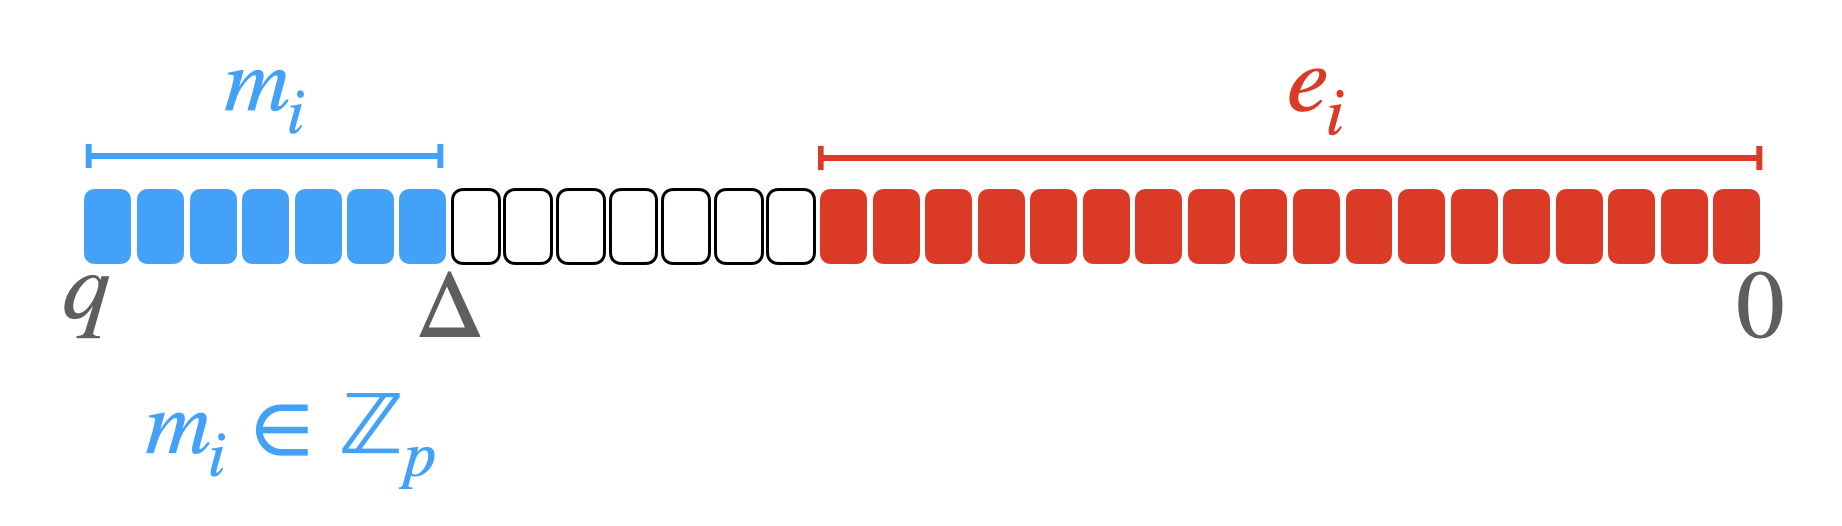
\includegraphics[width=1.0\textwidth]{figures/encryption-bit-visualization.png}
	\caption{\href{https://www.zama.org/post/tfhe-deep-dive-part-1}{Bitwise representation of LWE/RLWE/GLWE ciphertext.}}
	\label{fig:mesh1}
\end{figure}

Any FHE ciphertext (LWE, RLWE, GLWE etc. and other types) are can be represented as shown in the figure above. The ciphertext modulus (q) defines this number of bits (each bit is a small square in the figure). The blue squares are where the message is stored and as it can be seen, its stored in the MSBs (Most Significant Bits) here and its length is defined based on the value of plaintext modulus (p), while the noise (the red squares) is stored in the LSB (Least significant bits). Having $p=8 (2^3)$ and $q = 2^{32}$ means that that message would be stored in the first 3 bits out of the 32 bits which would be the length of the entire ciphertext. \newline

This is done by design. As defined above, during encryption of the plaintext by doing $m \cdot \Delta$, where $\Delta = \frac {q} {p}$, we are basically 'moving' our message from the $log_2p$ bit message to $log_2q$ message length, with the actual message taking the $log_2p$ MSBs. All the other values like q, e etc are also in the q space as well. The way the noise is constructed is such that it will always take the LSB spaces, as we take samples for a normal distribution such that these samples are <<1, which are then multiplied with q, which, while elevating the noise to this q, space, its still much smaller than the message encoding. Therefore, when they are added, we naturally get this structure shown in the figure above. \newline

The separation seen between the red and blue bits is very important for decryption to be accurate and exact. During decryption and decoding, the result of $b - \langle a, s \rangle$ is rounded down to the p space.  If the noise and actual message bits are not 'separated' like this, the rounding will not be accurate and will contain traces of noise, making decryption inaccurate. This is also the reason why you cant do a lot of chained addition and multiplication (multiplication even moreso) with ciphertexts as they increase the noise and it starts moving left. \newline

Following needs to be cared for to ensure this 'gap':
\begin{itemize}
	\item Ensure that $q >> p$.
	\item The standard deviation $\sigma$ should be small enough that the noise does not become too large (rememeber that we are multiplying the normal sample with q), in my experiments, where p = 8 and $q = 2^{32}$, I have used $\sigma = 2^{-20}$. However, $\sigma$ should not be so small that the noise becomes extremely small as that compromises with the security. (Note that Im not sure if the $\sigma$ that I've used is secure or no, I used it from a tutorial).
\end{itemize}

\subsection{Notes about encryption and decryption in Core-Crypto}
The core-crypto API in rust requires you to do a few shenanigans (technically theyre the 'correct' ways to do something like but Im a python pleb so Ill call it a shenanigan). The API actually works with only unsigned integers and thus, you cant just work with a negative number as is. You need to cast any signed integer (positive or negative) as the corresponding unsigned integer. Also, during decryption, in the decoding process, after performing mod wrt the plaintext modulus, do not forget to cast it back to the signed integer to get the correct answer.


\section{Arithmetic}
This section talks about how arithmetic is done in LWECiphertexts. The following operations are possible:
\begin{itemize}
  \item Addition: Ciphertext-ciphertext and Ciphertext-Plaintext addition.
  \item Subtraction: Same as addition.
        \item Multiplication: Ciphertext-plaintext multiplication. Multiplication between two ciphertexts isnt possible it seems.
\end{itemize}

\subsection{Addition}
An LWE ciphertext is defined as $(a, b)$, where $a \in \mathcal{Z}^n$ and $b \in \mathcal{Z}$. Since both a and b are going to be ramdom, we denote by $LWE_s(m)$, the family of ciphertexts that encrypt the cleartext message m under the secret key s.
\subsubsection{Ciphertext-Plaintext addition}
Say you want to add a ciphertext encrypting a cleartext message m, $L_1 = LWE_s(m) = (a, b) \in (\mathcal{Z}^n, \mathcal{Z})$, and a scalar, cosntant value c. We denote this operation by PAdd, such that $PAdd(L_1, c) = LWE_s(m+c)$. To add c to $L_1$, you do the following:
\begin{enumerate}
  \item Encode c by doing $\Delta \cdot c$.
  \item Add $\Delta \cdot c$ to b of $L_1$.
        \item The resulting ciphertext $(a, b + c)$ is the answer.
\end{enumerate}

\textbf{Why does this work?} \newline
To decrypt, $L_1 = (a, b)$ you do:
\begin{center}
  $b - \langle a, s \rangle = \Delta \cdot m + e$.\newline
  Followed by $\lfloor \frac{\Delta \cdot m + e}{\Delta} \rceil$ which gives the decrypted result m back.
\end{center}
Similarly, for $LWE_S(a, b+\Delta \cdot c)$:
\begin{center}
  $(b + \Delta \cdot c) - \langle a, s \rangle = \Delta \cdot m + \Delta \cdot c + e$ \newline
  Followed by $\lfloor \frac{\Delta (c + m) + e} {\Delta} \rceil$ which will give the decrypted result $(m + c)$ back.
\end{center}

\subsubsection{Ciphertext-Ciphertext Addition}
Consider two ciphertexts $L_0 = LWE_s(m_0)$ and $L_1 = LWE_s(m_1)$ encrypted under the same encryption key \textit{s}. You want to define a function $CAdd(L_0, L_1) = L_{sum}$ such that $Dec(L_{sum}) = (m_0 + m_1)$. If the ciphertexts are $L_0 = (a_0, b_0)$ and $L_1 = (a_1, b_1)$, then $L_{sum} = (a_0 + a_1, b_0 + b_1)$. \newline

\textbf{Why does this work?} \newline
Decrypting $L_{sum}$:
\begin{center}
	$(b_0 + b_1) - (a_0 + a_1) s = \Delta(m_0 + m_1) + (e_0 + e_1)$ \newline
	Dividing this by $\Delta$ and rounding will give the decrypted $m_0 + m_1$.
\end{center}
\textbf{Note on the noise increase}: As you can observe, the noise in the resulting ciphertext is higher as it is the sum of noise from both the added ciphertexts. This is expected, and while it does not increase noise a lot (as its only adding), you can still not do a lot of chained additions because after a point the noise becomes too large for proper decryption to happen. However, if your parameters are set correctly, this point is so far away that it is not a point of worry for most applications.

\subsection{Subtraction}
Subtraction works the same way you just replace the + by the -.

\subsubsection{Multiplication}
For LWE ciphertexts, only multiplication with a scalar is supported. Consider a ciphertext $L = LWE_s(m) = (a, b)$ encyrpting a message m, which is to be multiplied with a cleartext scalar c. We define a function $PMul(L, c) = LWE_s(c \cdot m)$, where $PMul(L, c) = (a \cdot c, b \cdot c)$.  \newline
\textbf{Why does this work?} \newline
Decrypting $PMul(L, c)$:
\begin{center}
	$b \cdot c - a \cdot c \cdot s = c ( m + e )$ \newline
	$b \cdot c - a \cdot s \cdot c = (c \cdot m) + (c \cdot e) $
\end{center}
Decoding this by dividing by $\Delta$ and rounding  will give $m \cdot c$.
\textbf{Code for LWECiphertext arithmetic:}
\begin{minted}[
	fontsize=\small,
	frame=single,
	framesep=3mm,
	bgcolor=bg
	]{python}
# LWECiphertext Class
	def add_ciphertext(self, other: LWECiphertext):
		'''
		This function adds a given ciphertext to the current ciphertext and returns a new ciphertext.
		'''
		# adding their as and bs
		added_a = np.add(self.a, other.a, dtype=np.int32)
		added_b = np.add(self.b, other.b, dtype=np.int32)
	
		# # taking mods just to see if this works, but we have to take mod wrt q
		# q = config.q
		# added_a = ((added_a + (q//2)) % q) - (q//2)
		# added_b = ((added_b + (q//2)) % q) - (q//2) # im getting overflow errors when doing this
		
		return LWECiphertext(added_a, added_b)
		
	def sub_ciphertext(self, other:LWECiphertext):
		'''
		This function subtracts the other ciphertext from the current one.
		'''
		sub_a = np.subtract(self.a, other.a, dtype=np.int32)
		sub_b = np.subtract(self.b, other.b, dtype=np.int32)
		return LWECiphertext(sub_a, sub_b)
	
	def mul_plaintext(self, other:np.int32):
		'''
		Multiply the other integer to current ciphertext
		'''
		# we just need to multiply the give plaintext to both a and b
		mul_a = np.multiply(other, self.a, dtype=np.int32)
		mul_b = np.multiply(other, self.b, dtype=np.int32)
		return LWECiphertext(mul_a, mul_b)
	
	def add_plaintext(self, other:LWEPlaintext):
		'''
		Add the other plaintext to the current ciphertext. This function assumes that the input plaintext message is already encoded to R_q.
		'''
		# we just need to scale other and then add it to b
		addb = np.add(self.b, other.m, dtype=np.int32)
		return LWECiphertext(self.a, addb)
\end{minted}

\section{Trivial LWE Ciphertext}
This is just a ciphertext (a, b) where a is a vector of zeros and b is just the encoded message with no noise added to it. It will be used down the line to enable RLWE ciphertext arithmetic.

% --- END OF CHAPTER 1 ---
\chapter{Working With Polynomials.}
	\section{Why do we need to use Polynomials?}
		So from what I've understood in my limited reading so far, whenever you do any operation in any kind of a FHE/HE scheme, including TFHE, the noise \textit{e} increases, it does so especially during multiplication. Now, that makes it not very practical when we want to chain operations together, and do operations that are more complex than regular arithmetic to  implement complex (relatively speaking) functions. However, there is another operation, called \textit{Bootstrapping}, which will be discussed in later chapters, which basically 'resets' this noise, thus allowing for chaining of complex operations in TFHE. Now for doing this bootstrapping operation, we want to work with polynomials as polynomials make it easy for us to implement bootstrapping.
		
	\section{Polynomial Ring and Negacyclic Rings}
		These are two terms that are used quite a lot and also form the basis of working with polynomials in TFHE. A polynomial ring is described/shown as follows:
		\begin{center}
			$R_q[x]/(x^N + 1)$
		\end{center}
		There are two separate things here, the first is $R_q[x]$, and the second is  $(x^N + 1)$. $R_q[x]$ means that for any polynomial that belongs to this ring, all of its coefficients are mod q, Meaning, if you define any polynomial as $p(x) = c_0 + c_1x + c_2x^2 + .... + c_nx^n$, its coefficients $[c_0, c_1, c_2, ..., c_n] \in R_q$, meaning they are in the range $[-\frac{q}{2}, \frac{q}{2})$. The $(x^N + 1)$ plays the same role here as q played for $R_q[x]/q$, but for the degree of polynomial this time, the polynomial that belongs in this ring is considered modulo $(x^N + 1)$. To make a polynomial modulo $(x^N + 1)$,  you just divide it with $(x^N + 1)$ and use the remainder. A polynomial can have an arbitrarily high degree, but taking a mod caps it to be less than N.\\
		Now why do we call it a ring? Like in a scalar ring, $Z/qZ$, where two scalars are equal modulo q if they differ by a multiple of q. Here as well, two polynomials are considered to be equal modulo $(x^N + 1)$ if they differ by a multiple of $(x^N + 1)$. \newline
		(\textit{Important Note: This distinction is something that I 'observed' from the literature that I read, it may or may not be exactly the truth (NOTE TO SELF: Dig deeper),  but nonetheless, I think its better to use this nomenclature as it helps differentiate.}) \newline		
		Coming to the \textit{negacyclic} thing, a polynomial who is modulo $(x^N + 1)$, basically 'loops' around to 1 once it's degree crosses N, but with a negative sign. For example, if you have N = 4, so $(x^N + 1)$ becomes $(x^4 + 1)$, and you have a polynomial $1 + x^5$, then:
		\begin{center}
			$1 + x^5 = 1 - x \:  (mod \: (x^N + 1))$ (1 - x is the remainder.) \\
			$x^8 + x^5 = x^2 - x \:  (mod \: (x^N + 1))$
		\end{center}
		As you can see, that as the degree of the polynomial got larger than N, the powers of x that were larger than N (4) basically just wrapped around to one, but with an opposite sign. ($ x^5$ became $x$, $x^8$ became $x^2$). This is what negacyclic means, and this is the behavior of polynomials in a ring. In fact, this can also be used as a "trick" to calculate a polynomial modulo $(x^N + 1)$, you just replace all instances of $x^N$ by -1, and you will get the modulo N version of that polynomial. Note that for any operations done between two polynomials that are in the ring, the result will also be modulo $(x^N + 1)$. Example: Consider two polynomials $f(x) = 1 + x^3$ and $g(x) = x^2$, and they're in the ring $Z_q[x]/(x^4 + 1)$, then $f(x) \cdot g(x)$ will be:
		\begin{center}
			$f(x) \cdot g(x) = x^2 + x^5 = x^2 - x \: (mod \: (x^N + 1))$
		\end{center}
		
		One very important thing to realize and understand is that when we say that a polynomial being in a ring $R_q[x]/(x^N + 1)$, it doesn't mean that it can not have a degree $> N$, it can. However, the process of doing modulus $x^N + 1$ the degree gets reduced to a number that smaller than N. Try to relate it to plaintext modulus, when we say that we have a number x s.t. $x \in R_q$,  it also means that any number that is beyond the range $[-\frac{q}{2}, \frac{q}{2})$, can be represented as another number that is in that range. Meaning, integers that are within that range, sort of act as a 'representative integer' for everything outside of that range who have the same mod q. Similarly, any polynomial \textit{f(x)} that is in the ring, sort of represents a family of polynomials that have the same modulus $R_q[x]/(x^N + 1)$. This is a very subtle thing that I understood and is something that is important conceptually. So whenever we talk about a polynomial $f(x) \in R_q[x]/(x^N + 1)$, f(x) really represents a family of polynomials that would share the same mod, and not just a specific polynomial.

\begin{minted}[
	fontsize=\small,
	frame=single,
	framesep=3mm,
	bgcolor=bg
	]{python}
class Polynomial:
	'''
	This class represents a polynomial in the ring Z_q[x]/(x^n + 1)
	Note that the coefficients here are in increasing order of degrees of x, [constant, x, x**2, ..., x**N]
	'''
	
	def __init__(self, N, coeffs: np.ndarray):
		self.N = N
		self.coeffs = coeffs
	
	def __str__(self):
		'''
		Print the ciphertext as an equation.
		'''
		prtstr = ""
		nonzeroct = 0
		for i, c in enumerate(self.coeffs):
			if c:
				if nonzeroct:
					prtstr += " + "
				prtstr += f"{c}x^{i}"
				nonzeroct += 1
		
		return prtstr
	
	def polynomial_const_multiply(self, c:np.int32):
		'''
		Multiply the current polynomial with the given constant integer and return it as a new polynomial.
		'''
		new_p = Polynomial(self.N, np.multiply(c, self.coeffs, dtype=np.int32))
		return new_p
	
	def polynomial_multiply(self, p2: Polynomial):
		'''
		Multiply the current polynomial with the given poylnomial and return the new polynomial.
		'''
		# get the N from p2
		p2N = p2.N
		# multiply and pad the results to have 2N-1 (thats the longest polynomial you can get)
		# the np.polymul function requires the coefficients in decreasing order of powers or x, se we reverse the current coeff array and then reverse the final output's back again.
		poly_prod = np.polymul(self.coeffs[::-1], p2.coeffs[::-1])[::-1]
		# creating the final answer with padded coeffs
		poly_padded = np.zeros(2*self.N - 1, dtype=np.int32)
		poly_padded[:poly_prod.shape[0]] = poly_prod
		
		# now, taking modulus of the result (poly_padded) wrt x^N + 1
		result = poly_padded[:self.N]
		result[:-1] -= poly_padded[self.N:]
		return Polynomial(self.N, result)
	
	def polynomial_add(self, p2: Polynomial):
		'''
		This function adds a polyonmial to the given polynomial and returns the output as a new polynomial.
		'''
		add_coeffs = np.add(self.coeffs, p2.coeffs, dtype=np.int32)
		return Polynomial(self.N, add_coeffs)
		
	def polynomial_subtract(self, p2: Polynomial):
		'''
		This function subtracts the given polynomial from the current one and returns the new polynomial.
		Note: Its self - p2 and not p2 - self.
		'''
		sub_coeffs = np.subtract(self.coeffs, p2.coeffs, dtype=np.int32)
		return Polynomial(self.N, sub_coeffs)
	
def make_zero_polynomial(N:int):
	'''
	Declare a zero polynomial and return it. Basically a polynomial where all the coefficients are zeros.
	'''
	return Polynomial(N = N, coeffs = np.zeros(N, dtype=np.int32))
	
def build_monomial(N, i, c):
	'''
	This function builds a monomial c * x^i in the ring R[x]/(x^N + 1)
	NOTE: Rememeber that the coeffs are in increasing order of powers of x. [constant, x, x**2, ..., x**N]
	'''
	coeffs = np.zeros(N, dtype=np.int32)
	
	# find k such that 0 <= i + k*N < N
	i_mod_n = i % N
	k = (i_mod_n - i)//N
	
	# if k is odd then the monomial gets a negative sign because
	# x^i = (-1)^k + x^(i + k*N) = (-1)^k + x^(i % N)
	sign = 1 if k % 2 == 0 else -1
	coeffs[i_mod_n] = sign * c
	
	return Polynomial(N, coeffs)
\end{minted}
		
	\section{RLWE Ciphertexts}
		Like LWE Ciphertexts encrypt scalar values, RLWE Ciphertexts encrypt polynomials. Meaning, the following things change in RLWE Ciphertexts compared to LWE CIphertexts.
		\begin{itemize}
			\item  The secret key here becomes a polynomial with degree N-1 instead of a vector. Again, one way of creating a secret key can be having a polynomial with binary coefficients, meaning, $s(x) = s_0 + s_1x + s_2x^2 + ... + s_{N-1}x^{N-1}$.
			\item a is now a polynomial too, instead of a vector.
			\item b is a polynomial instead of a scalar value.
		\end{itemize}
		However, the encryption process remains the same. Also, the configurations, p (plaintext modulus), q (ciphertext modulus) and the std deviation ($\sigma$) remain the same. The parameter N which was used to define the legnth of the encryption key and a, are now used as the degree of the secret key s(x) and a(x) polynomials.
		\begin{minted}[
			fontsize=\small,
			frame=single,
			framesep=3mm,
			bgcolor=bg
			]{python}
class RLWEConfig:
	'''
	This class defines the RLWE config.
	'''
	def __init__(self, N, p, q, sigma):
		self.N = N
		self.p = p
		self.q = q
		self.sigma = sigma
		\end{minted}

\begin{minted}[
	fontsize=\small,
	frame=single,
	framesep=3mm,
	bgcolor=bg
	]{python}
class RLWEEncryptionKey:
	'''
	This class defines the RLWE encryption/secret key and performs encryption and decryption of ciphertexts.
	'''
	def __init__(self, config:RLWEConfig):
		self.config = config
		self.key = Polynomial # this time, the key is also a polynomial.
		
	def generate_key(self):
		'''
		Generate the key. The key is a random polynomial of degree N with binary coefficients.
		'''
		self.key = Polynomial(
			N=self.config.N,
			coeffs = np.random.randint(
					low = 0,
					high = 2,
					size = self.config.N,
					dtype = np.int32
				)
			)
\end{minted}
		
		\subsection{Encoding}
			To encode a cleartext polynomial into plaintext, you encode the individual coefficients the same way a scalar is encoded for LWE. After encoding a polynomial $p(x) = c_0 + c_1x + c_2x^2 + ... + c_{N-1}x^{N-1}$ becomes $p'(x) = c'_0 + c'_1x + c'_2x^2 + ... + c'_{N-1}x^{N-1}$, where $c'_i = c_i \cdot \Delta; \: \forall i \in [0, N-1]$ where $\Delta = \frac{q}{p}$.
\begin{minted}[
	fontsize=\small,
	frame=single,
	framesep=3mm,
	bgcolor=bg
	]{python}
def encode_rlwe(p: Polynomial, config: RLWEConfig):
	'''
	This function encodes the cleartext polynomial and returns it as a Plaintext.
	'''
	# get the delta
	delta = config.q//config.p
	# scale each coefficient of the polynomial by multiplying it with delta
	scaled_coeffs = np.multiply(p.coeffs, delta, dtype=np.int32)
	return RLWEPlaintext(Polynomial(p.N, scaled_coeffs), config=config)
\end{minted}

\begin{minted}[
	fontsize=\small,
	frame=single,
	framesep=3mm,
	bgcolor=bg
	]{python}
class RLWEPlaintext:
	'''
	This class implements the RLWE Plaintext. This just stores the encoded message polynomial. Functionally, it isnt really needed but Ive just added it to make my code consistent with how TFHE libraries work.
	'''
	def __init__(self, p: Polynomial, config: RLWEConfig):
		self.p = p
		self.config = config
\end{minted}
			
		\subsection{Encryption}
			An RLWE encryption of a polynomial p(x) under the secret key s(x) is a tuple (a(x), b(x)). Such that: \newline
			\begin{center}
				$b(x) = a(x) \cdot s(x) + p'(x) + e(x)$
			\end{center}
			where $a(x) \cdot s(x)$ is the polynomial multiplication between a(x) and s(x) mod $(x^N + 1)$. e(x) is the noise polynomial whose coefficients are created in the same way the noise e was created for LWE ciphertexts. a(x) is also a polynomial whose coefficients are created the same way the vector a was created for LWE ciphertexts. Note that the p'(x) here is the encoded polynomial (plaintext) and not the raw polynomial (cleartext).
			Now since RLWE encryptions are random, as elements of it such as a(x) and e(x) are generated randomly, a family of RLWE ciphertexts that encrypt a polynomial p(x) under the secret key s(x) is denoted by: $Enc^{RLWE}_{s(x)} ( p(x)) = \langle a(x), b(x) \rangle$. Note that sometimes $RLWE_{s(x)}(p(x))$ might be used to refer to them as well just because its easier and faster to write.\newpage
		
\begin{minted}[
	fontsize=\small,
	frame=single,
	framesep=3mm,
	bgcolor=bg
	]{python}
def rlwe_generate_uniform_sample(config: RLWEConfig) -> Polynomial:
	'''
	This function generates a polynomial of the degree specified in the config where each coefficient is an integer sampled from a uniform random distribution.
	'''
	# get the limits
	minval = -config.q//2
	maxval = config.q//2
	
	# generate N values between the min (inclusive) and max (exclusive)
	coeffs = np.random.randint(minval, maxval, size=config.N, dtype=np.int32)
	
	return Polynomial(config.N, coeffs=coeffs)
	
def rlwe_generate_normal_sample(config: RLWEConfig) -> Polynomial:
	'''
	This function generates a polynomial of the degree as per the config where each coefficient is drawn from a normal distribution with mean 0 and standard distribution given in the config.
	'''
	coeffs = np.int32(np.multiply(np.random.normal(0, config.sigma, size=config.N), config.q//2))
	return Polynomial(config.N, coeffs)
\end{minted}

\begin{minted}[
	fontsize=\small,
	frame=single,
	framesep=3mm,
	bgcolor=bg
	]{python}
# RLWECiphertext Class...
def encrypt(self, mx: RLWEPlaintext):
	'''
	Encrypt the input Polynomial p into an RLWE Ciphertext.
	'''
	# generate a and noise e
	a = rlwe_generate_uniform_sample(self.config)
	e = rlwe_generate_normal_sample(self.config)
	
	# encrypting
	a_times_s = a.polynomial_multiply(self.key) # <a, s>
	as_plus_m = a_times_s.polynomial_add(mx.p) # <a, s> + m (m is already encoded, which is why I wrote m and not delta * m)
	b = as_plus_m.polynomial_add(e)
	
	return RLWECiphertext(a, b, self.config)
...
\end{minted}

\begin{minted}[
	fontsize=\small,
	frame=single,
	framesep=3mm,
	bgcolor=bg
	]{python}
class RLWECiphertext:
'''
	This class implements the RLWE ciphertext.
	'''
	def __init__(self, a: Polynomial, b: Polynomial, config: RLWEConfig):
		self.config = config
		self.a = a
		self.b = b
\end{minted}
			
		\subsection{Decryption}
			The decryption also is similar to the LWE decryption. You first do:
			\begin{center}
				$b(x) - a(x) \cdot s(x) =  p'(x) + e(x)$
			\end{center}
			After that, you round and decode the $p'(x) + e(x)$ to get p(x).\newline
			\textbf{Decoding}\newline
				To decode the obtained $p'(x) + e(x)$, you just do $\frac{p'(x) + e(x)}{\Delta}$ to finally get p(x).
\begin{minted}[
	fontsize=\small,
	frame=single,
	framesep=3mm,
	bgcolor=bg
	]{python}
def decode_coeff(c, delta, p):
	'''
	This function decodes a specific coefficient within the polynomial.
	'''
	# divide by delta and round
	decoded_c = int(np.rint(c/delta))
	# calculate decoded_c mod p and you get the final decoded value
	out = ((decoded_c + (p//2)) % p) - (p//2)
	return out
	
def decode_rlwe(p: Polynomial, config: RLWEConfig):
	'''
	This function decodes the given polynomial to remove the noise and get the final decrypted cleartext.
	'''
	# calcualte the delta
	delta = config.q//config.p
	raw_coeffs = p.coeffs
	# decoded each coeff and get the output polynomial
	decoded_coeffs = np.array([decode_coeff(c, delta,config.p) for c in raw_coeffs])
	
	return Polynomial(config.N, decoded_coeffs)
\end{minted}

\begin{minted}[
	fontsize=\small,
	frame=single,
	framesep=3mm,
	bgcolor=bg
	]{python}
# RLWEEncryptionKey Code...
	def decrypt(self, cx: RLWECiphertext) -> Polynomial:
		'''
		Decrypt the given ciphertext, decode it and return the cleartext polynomial.
		'''
		# separate a and b
		ca = cx.a
		cb = cx.b
		# subtracting <a, s> from b
		subbed = cb.polynomial_subtract(ca.polynomial_multiply(self.key))
		# decode: divide by delta to remove the noise and take mod wrt p
		decoded = decode_rlwe(subbed, self.config)
		
		return decoded
\end{minted}
			
		\subsection{Switching Between LWE and RLWE Encryption Keys}
		Remember that LWE encryption key is a vector of integers (for example, binary values), while RLWE encryption key is a polynomial with integer coefficients (binary coefficients for instance). it is possible and very trivial to switch an LWE key to RLWE key. To do this, you just use the N length vector key from LWE as coefficients for s(x), the RLWE key. It is important to remember that this will only work and should be done only when the configuration parameters for both the schemes are exactly the same.
\begin{minted}[
	fontsize=\small,
	frame=single,
	framesep=3mm,
	bgcolor=bg
	]{python}
def lwe_to_rlwe_key(lwe_key: LWEEncryptionKey, config: RLWEConfig):
	'''
	This function creates an RLWE key for/from the given RLWE key.
	'''
	# creating a polynomial with the coeffs as the lwe_key
	if lwe_key.config.n != config.N:
	raise ValueError("The size of LWEKey and degree of RLWEConfig do not match.")
	key_poly = Polynomial(N=config.N, coeffs=lwe_key.key)
	rlwe_key = RLWEEncryptionKey(config=config)
	rlwe_key.key = key_poly
	
	return rlwe_key
\end{minted}
		
		\subsection{Arithmetic}
		Again, just like LWE ciphertexts, there are three types arithmetic operations that can be done with RLWE ciphertexts:
		\begin{itemize}
			\item Ciphertext Addition and Subtraction: CAdd, and CSub
			\item Plaintext Addition and Subtraction: PAdd and PSub
			\item Plaintext - Ciphertext Multiplcation: PMul
			\item Multiplying two RLWE ciphertexts is not trivially possible. There are ways to do ciphertext multiplication, between an RLWE ciphertext and something called a GSW ciphertext, which will be discussed in the coming chapters.
		\end{itemize}
		
		\subsubsection{1. Ciphertext Addition and Subtraction}
			This section primarily describes how ciphertext addition is done. Subtraction is done the same way, except there you subtract instead of add (sounds silly but will make sense soon). Adding two ciphertexts $R_1 = RLWE_{s(x)}(f_1(x))$ and $R_2 = RLWE_{s(x)}(f_2(x))$ encrypting $f_1(x)$ and $f_2(x)$ is denoted by CAdd($R_1$, $R_2$) and it returns an RLWE ciphertext encrypting $f_1(x) + f_2(x)$.
			\begin{center}
				$R_1 = \langle a_1(x), b_1(x) \rangle$ and $R_2 = \langle a_2(x), b_2(x) \rangle$\\
				CAdd($R_1 + R_2$) = $\langle a_1(x) + a_2(x), b_1(x) + b_2(x) \rangle = RLWE_{s(x)} (f_1(x) + f_2(x))$
			\end{center}
			
			Similarly, the CSub operation returns RLWE encryption of two ciphertext, here, as the description said, you need to replace the + sign with the - sign. The process remains the same.
			
		\subsubsection{2. Plaintext - Ciphertext Addition and Subtraction}
		This section discusses addition and subtraction between plaintexts and ciphertexts. This describes plaintext addition in detail. Just like the ciphertext-ciphertext version, the subtraction follows the same steps but replaces the + sign for a - sign. The plaintext-ciphertext addition operation is defined as PAdd(R, P), where R is an RLWE Ciphertext encrypting a polynomial f(x) and P is an RLWE plaintext that encodes another polynomial $f_2(x)$. The operation PAdd returns a new RLWE ciphertext that encrypts $RLWE_{s(x)}(f(x) + p(x))$. Remember that an RLWE Ciphertext, $RLWE_{s(x)}(f(x)) = \langle a(x), b(x) \rangle$. Then, PAdd returns a new RLWE ciphertext $\langle a(x), b(x) + p(x) \rangle$.
		
		\subsubsection{3. Plaintext - Ciphertext Multiplication}
		The operation PMul(R, P) multiplies an RLWE ciphertext $R = RLWE_{s(x)} (f(x))$ and an RLWE plaintext p(x) and returns a new RLWE Ciphertext $RLWE_{s(x)} (f(x) \cdot p(x))$. Please note that while it says plaintext multiplication (which Im also using to be consistent with the literature everywhere), the polynomial p(x) isnt encoded, its just the raw cleartext polynomial p(x) which is multiplied. Recall that the RLWE  ciphertext is $R = \langle a(x), b(x) \rangle$. The multiplication is done by multiplying both a(x) and b(x) by the polynomial p(x). Note that this is a polynomial multiplication and not a pointwise multiplication and its done mod $(x^N + 1)$. Therefore:
		\begin{center}
			$PMul(R, P) = \langle a(x) \cdot p(x), b(x) \cdot p(x) \rangle$
		\end{center}
		\textbf{Why did we just use cleartext p(x) and not encode it}\\
		Remember that the ciphertext encrypts an encoded polynomial, whose coefficients are already multiplied by $\Delta$. Encoding the plaintext polynomial and then multiplying will result in the resulting polynomial being 're-encoded', meaning, it becomes $(\Delta \cdot f(x)) \cdot (\Delta \cdot p(x)) = \Delta^2 \cdot f(x) \cdot p(x)$ which will mess up with the decryption. Therefore, we just need only one of the two encoded and since one of them is a ciphertext, its already encoded by design and thus, the other one should be left as cleartext. This is important to remember as literature uses plaintext multiplication and the terminology might give an incorrect impression.
\begin{minted}[
	fontsize=\small,
	frame=single,
	framesep=3mm,
	bgcolor=bg
	]{python}
# RLWECiphertext Code...
	def add_ciphertext(self, other: RLWECiphertext):
		'''
		Add another ciphertext <other> to the current ciphertext and return the result as a new ciphertext. Two add two ciphertexts, you just add their respective a and b polynomials.
		'''
		# adding a and b, and creating a new ciphertext
		added_a = self.a.polynomial_add(other.a)
		added_b = self.b.polynomial_add(other.b)
		
		return RLWECiphertext(added_a, added_b, self.config)
		
	def sub_ciphertext(self, other: RLWECiphertext):
		'''
		Subtract another ciphertext <other> from the current one and return the result as a new ciphertext. This operation subtracts <other> from the <self> and not the other way round.
		'''
		# subtracting a and b and returning a new ciphertext
		subbed_a = self.a.polynomial_subtract(other.a)
		subbed_b = self.b.polynomial_subtract(other.b)
		
		return RLWECiphertext(subbed_a, subbed_b, self.config)
	
	def mul_plaintext(self, cx: RLWEPlaintext):
		'''
		This function multiplys the given plaintext to self and returns the product as a new ciphertext.
		'''
		# for this, you multiply both a and b with the plaintext
		mul_a = self.a.polynomial_multiply(cx.p)
		mul_b = self.b.polynomial_multiply(cx.p)
		
		return RLWECiphertext(mul_a, mul_b, self.config)
\end{minted}
		
	\subsection{Trivial RLWE Ciphertext}
	A trivial RLWE ciphertext is an RLWE ciphertext where a(x) is just a zero polynomial and b(x) is just the encoded plaintext.
\begin{minted}[
	fontsize=\small,
	frame=single,
	framesep=3mm,
	bgcolor=bg
	]{python}
def get_trivial_rlwe_ciphertext(mx: Polynomial, config: RLWEConfig):
	'''
	This function returns the trivial RLWE ciphertext for the given config. Trivial RLWE ciphertext is basically just an RLWE ciphertext where a is just a zero polynomial and b is polynomial itself.
	NOTE: Im not very sure if we should encode the input polynomial, meaning, if we take a cleartext input or plaintext input.
	'''
	# sanity check
	if len(mx.coeffs) != config.N:
	raise ValueError("The polynomial has a degree thats different from the degree provided in the config file. Please ensure that theyre the same.")
	# creating a
	a = make_zero_polynomial(config.N)
	return RLWECiphertext(a = a, b = mx, config=config)
\end{minted}

\chapter{GSW Ciphertexts and Ciphertext Multiplication}
	The previous section mentioned that multiplication between two RLWE ciphertexts is non-trivial. Instead, one way of multiplying two ciphertexts is multiplication between an RLWE and a GSW ciphertext. This chapter first describes GSW Ciphertext and then proceeds to talk about multiplying a GSW and an RLWE ciphertext together..
	
	\section{Base-p Representation}
	For ciphertexts, a polynomial's coefficients are encoded to the 'q-space', meaning that the coefficients will be in the range $[-\frac{q}{2}, \frac{q}{2})$. For the base-p representation, we define a parameter p (note that its not the same as the plaintext modulus p, anywhere in this section p will be used to denote p for base-p and the plaintext modulus will be pt), and $Z_p$ denotes the range for elements to be in the range $[-\frac{p}{2}, \frac{p}{2})$. The base-p representation of a given integer $x \in Z_q$ will be a series of integers $(x_0, x_1, ..., x_k)$ such that:
	\begin{center}
		$x = x_0 + x_1 \cdot p + x_2 \cdot p^2 + ... + x_{k-1} \cdot p^{k-1}$
	\end{center}
	For example, if we want to find the base-p representation of say x = 256 for $p = 2^8 = 256$ will be [0, 1, 0, 0].\\
	For x = 1000, it will be [-24, 4, 0, 0] (these are the vales of xis).
	
	\subsection{How are these calculated?}
	\begin{itemize}
		\item To calculate the base-p representation of any integer, we need to find the length of the sequence. This is denoted by k and is calculated as $k = \frac{log_2 q}{log_2 p}$.
		\item After that, the easiest way to find the k integers for this representation is:
		\begin{itemize}
			\item Get the binary representation of the integer. Even if the representation takes less than $log_2 q$ bits, it should be expanded to fit the length.
			\item Then, divide this representation into k chunks of length $log_2 p$.
			\item Each chunk converted into its integer representation will be the k-th element of the representation. Note that the sequence will start from the right hand side.
		\end{itemize}
	\end{itemize}
\begin{minted}[
	fontsize=\small,
	frame=single,
	framesep=3mm,
	bgcolor=bg
	]{python}
def get_k(q, p):
	'''
	Given q (ciphertext modulus) and p (not plaintext modulus, but a different parameter specifically for base p representation used for ciphertext-ciphertext multiplication of an RLWE and GWE cipherterxts), get the value of k, which is the sequence length of base-p representation of any input.
	'''
	return np.int32(np.log2(q)/np.log2(p))
\end{minted}
	The problem with the above method to find the base-p representation is that it works with unsigned integers, as binary representation loses the sign and the elements of the representation will also be unsigned. But FHE works with signed integers. While this technique cant be used as-is, it can be used after making a small modification to the original integer.  Basically, instead of finding the base-p representation of the integer x, it is offset by an integer B, and the above mentioned method is used to then calculate the base p representation of x + B. Let the representation be $(x'_0, x'_1, ..., x'_{k-1})$. Once it is obtained, $\frac{p}{2}$ can be subtracted from the individual elements of the sequence to get the base-p representation of x.
	
	\subsubsection{How to find the offset value?}
	We know that due to the property of base-p representations,
	\begin{center}
		$x = (x'_0 - \frac{p}{2}) + (x'_1 - \frac{p}{2}) \cdot p + (x'_2 - \frac{p}{2})\cdot p^2 + ... + (x'_{k-1} - \frac{p}{2})\cdot p^{k-1}$ \newline
		
		$x = \sum\limits_{i=0}^{k-1} (x'_i - \frac{p}{2}) \cdot p^i  = \sum\limits_{i=0}^{k-1} x'_i \cdot p^i - \frac{p}{2} \sum\limits_{i=0}^{k-1} p^i$ 
	\end{center}
	
	Rearranging this, we get,
	\begin{center}
		$x + \frac{p}{2} \cdot \sum\limits_{i=0}^{l-1} p^i = \sum\limits_{i=0}^{k-1} x'_i \cdot p^i$
	\end{center}
	
	Based on this, $B = \frac{p}{2} \sum\limits_{i=0}^{k-1} p^i$
\begin{minted}[
	fontsize=\small,
	frame=single,
	framesep=3mm,
	bgcolor=bg
	]{python}
def convert_array_to_base_p(a: np.ndarray, p, q):
	'''
	This function converts each element into a its base p-representation, given the values of q (ciphertext modulus) and p (not plaintext modulus). Note that the representation for each element in a will be a sequence of a fixed length.
	'''
	log_p = np.log2(p).astype(np.int32)
	k = get_k(q = q, p = p)
	p_half = p//2
	offset = p_half * np.sum([p**i for i in range(k)])
	mask = p - 1 # this in binary is exactly log_p ones.
	
	a_offset = np.uint32(a + offset) # need to set this to uint 32 as the the p-bit representation will be calculated from unsigned integers and then converted to signed
	# return a_offset
	
	output = [] # this will store the output base-p representation for each element
	# NOTE: output is a list of k numpy arrays. Each numpy array stores the ith p-bit representation of the corresponding original input.
	for i in range(k):
	output.append(
	(np.right_shift(a_offset, i * log_p) & mask).astype(np.int32) - np.int32(p_half)
	)
	
	return output
	
def convert_base_p_to_int_array(a: Sequence[np.array], p: np.int32):
	'''
	This function takes as input the p-bit representations of an array, and converts it back into integer. a should be a list or a iterator of ndarrays where each ndarray contains the ith p-bit representation of the integer.
	'''
	# calculate x from the representation: x = x_0 + x_1 p + ... + x_k-1 p^k-1
	decimal_repr = np.zeros(len(a[0]), dtype=np.int32)
	for i in range(len(a)):
	decimal_repr += (a[i] * (p**i)).astype(np.int32)
	return decimal_repr
	
	# defining base p representation functions for polynomials
def get_base_p_from_polynomial(poly: Polynomial, p: np.int32, q: np.int32) -> Sequence[Polynomial]:
	'''
	This function converts each coefficient of the coefficients of the given polynomial and returns them as a set of polynomials (sequence of the polynomials is very important).
	'''
	coeffs = poly.coeffs
	# converting coeffs into base p representation
	coeffs_base_p = convert_array_to_base_p(coeffs, p, q)
	# create a polynomial for each array
	base_p_poly = [Polynomial(N=poly.N, coeffs = ic) for ic in coeffs_base_p]
	
	return base_p_poly
	
def get_poly_from_base_p(base_p_polys: Sequence[Polynomial], p) -> Polynomial:
	'''
	This function calculates the polynomial from the given base p representation polynomials.
	'''
	# get all the coefficients from the sequence
	base_p_coeffs = [p.coeffs for p in base_p_polys]
	# get the integer coeffs from the list
	int_coeffs = convert_base_p_to_int_array(base_p_coeffs, p)
	return Polynomial(N=base_p_polys[0].N, coeffs = int_coeffs)
\end{minted}
	
	\subsubsection{Why is the Base-p representation needed?}
	The base-p representation will be needed to perform the GSW encryption down the line which will be used for multiplication.
	
	\section{GSW Encryption}
	The idea behind a GSW encryption is to 'hide/mask' a plaintext polynomial f(x) between \textbf{zero ciphers} to encrypt it and hide it. 
\begin{minted}[
	fontsize=\small,
	frame=single,
	framesep=3mm,
	bgcolor=bg
	]{python}
class GSWConfig:
	'''
	This class implements the GSW Config. It takes the RLWE config, as most of the configurations are identical. Additionally, it also takes gsw_p, which will be used for the base p representation.
	'''
	def __init__(self, rlwecfg: RLWEConfig, gsw_p: int):
		self.rwlecfg = rlwecfg
		self.gsw_p = gsw_p
\end{minted}
	
	\begin{itemize}
		\item \textbf{Zero Cipher (RLWE):} A zero cipher is just the RLWE encryption of 0. Note that it is an actual encryption where the input cleartext (and thus the resulting plaintext) are 0, however, it still uses the entire encryption mechanisms and thus, the polynomials a(x) and b(x) are not zero. Remember this detail because in my experience, it becomes easy to mistake it for something thats more like a trivial RLWE encryption otherwise.
	\end{itemize}
	
	Let $Z_0, Z_1 \in RLWE_{s(x)} (0)$ be two RLWE zero ciphers, and Z be a 2x2 matrix whose i-th row is $Z_i$ (the matrix has 2 columns if you count a(x) and b(x) as separate columns, which is whats being done here.)
	\begin{center}
		$Z = \begin{pmatrix}
			Z_1 \\
			Z_2
		\end{pmatrix}$
	\end{center}
	And let the 2 x 2 identity matrix $I_{2 \times 2} = \begin{pmatrix}
		1 & 0\\
		0 & 1
	\end{pmatrix}$\newline
	
	The GSW ciphertext of a given polynomial is then given by:
	\begin{center}
		$Enc_{s(x)} ^{GSW}(f(x)) = f(x) \cdot I_{2 \times 2} + Z$
	\end{center}
	
\begin{minted}[
	fontsize=\small,
	frame=single,
	framesep=3mm,
	bgcolor=bg
	]{python}
class GSWConfig:
	'''
	This class implements the GSW Config. It takes the RLWE config, as most of the configurations are identical. Additionally, it also takes gsw_p, which will be used for the base p representation.
	'''
	def __init__(self, rlwecfg: RLWEConfig, gsw_p: int):
		self.rwlecfg = rlwecfg
		self.gsw_p = gsw_p
\end{minted}
\begin{minted}[
	fontsize=\small,
	frame=single,
	framesep=3mm,
	bgcolor=bg
	]{python}
class GSWCiphertext:
	'''
	This class implements the gsw ciphertext.
	'''
	def __init__(self, config: GSWConfig, polys: Sequence[RLWECiphertext]):
		self.config = config
		self.polys = polys
\end{minted}

\begin{minted}[
	fontsize=\small,
	frame=single,
	framesep=3mm,
	bgcolor=bg
	]{python}
class GSWEncryptionKey:
	'''
	This class implements the GSW encryption key and methods to encrypt and (possibly) decrypt a gsw ciphertext.
	'''
	def __init__(self, config: GSWConfig):
		self.config = config
		self.key = Polynomial # this is just going to be the RLWE encryption key s(x)
		self.rlwe_key = RLWEEncryptionKey
	
	def generate_key_from_rlwe_key(self, rlwe_key: RLWEEncryptionKey):
		'''
		This function creates the GSWEncryptionKey from the RLWEEncryption key. To be honest, its just the RLWEEncryption key as it is, but for the sake of structure of code and to keep it consistent with other classes. Its a little silly to save both the rlwe_key object and the key polynomail as well, but eh...
		'''
		self.key = rlwe_key.key
		self.rlwe_key = rlwe_key
	
	def get_rlwe_key_from_gsw(self):
		'''
		This function returns the rlwe key from the current gsw_key. Again, its the same, but consistency, formality, something, something...
		'''
		rlwe_key = RLWEEncryptionKey(config=self.config.rwlecfg)
		rlwe_key.key = self.key
		return rlwe_key
		
	def encrypt(self, fx: Polynomial):
		'''
		Encrypt a given polynomial as a GSWCiphertext.
		'''
		# first, we need to get the value of k
		k = get_k(self.config.rwlecfg.q, self.config.gsw_p)
		gsw_p = np.int32(self.config.gsw_p) # i dont want to write the whole thing
		# make Z: the zero encryption array of shape (2k, 2), note that each row is a RLWE ciphertext, the 2 just means (a(x), b(x))
		zero_poly = make_zero_polynomial(self.config.rwlecfg.N)
		zero_poly_plain = encode_rlwe(zero_poly, self.config.rwlecfg) # while for 0 config, the coefficients for both the plaintext and ciphertext are going to be the same, the encryption for RLWE only accepts an RLWEPlaintext and not a Polynomial
		Z = [
		self.rlwe_key.encrypt(zero_poly_plain) for _ in range(2*k)
		] # this has shpae (2k, 2)
		# create the GSW ciphertext
		# its created using the equation: fx * B_p + Z
		# i will implicitly divide the Z matrix in two halves 
		# here, ill iterate for k times, and for each iteration, the corresponding index's RLWE of the first half's a gets fx * (p**i) added and the corresponding index of the second half's b gets the same added
		for i in range(k):
			# multiply fx with the correct power of p
			scaled_fx = fx.polynomial_const_multiply(gsw_p**i)
			# add it to first half's a
			Z[i].a = Z[i].a.polynomial_add(scaled_fx)
			# add it to second half's b
			Z[i + k].b = Z[i + k].b.polynomial_add(scaled_fx)
		
		return GSWCiphertext(self.config, Z)
\end{minted}

	This results in a \textbf{vector} of two RLWE ciphertexts (note that it says vector of 2 RLWE ciphertexts, while Z is denoted as a matrix, each row there is an RLWE ciphertext, so it is also a vector to 2 RLWE ciphertexts. The reason for this weird seeming notation will be clear later.). There are a few thing to be noted about GSW ciphertext/encryption:
	\begin{itemize}
		\item The multiplication between f(x) and the identity matrix is pointwise.
		\item GSW ciphertext doesnt have to be a vector of just two RLWE ciphertexts, it can be arbitrarily long, just that each element of this vector has to be an RLWE ciphertext. In the coming section(s), a much longer GSW ciphertext will be created.
	\end{itemize}
	
	\section{RLWE - GSW Multiplication}
	\subsection{CMul: Basic Idea}
	If you have two polynomials g(x) and f(x), with an RLWE ciphertext $R = Enc^{RLWE}_{s(x)} (f(x))$ and a GSW ciphertext $G = Enc^{GSW}_{s(x)}(g(x))$, the there is a function CMul such that:
	\begin{center}
		$R_{prod} = CMul(R, G) = G \cdot R$
	\end{center}
	And CMul returns an RLWE ciphertext that encrypts $f(x) \cdot g(x)$.  Looking further into CMul:
	\begin{center}
		$R_{prod} = R \cdot ( g(x) \cdot I_{2 \times 2} + Z)$
	\end{center}
	This method will work as long as the coefficients of a(x), b(x) and g(x) are small. Based on the definition of GSW encryption, the polynomial g(x) will have (relatively) small coefficients (as its not really being encoded or encrypted), however, since f(x) is being encrypted into RLWE ciphertexts, coefficients of a(x) and b(x) will be very large. To decrease these magnitudes, one of the simplest ways can be by just multiplying it with $\frac{1}{p}$, where p >1, this will scale the coefficients of both a(x) and b(x) down and satisfy the condition. To compensate for the the GSW ciphertext can be scaled up and defined like so:
	\begin{center}
		$G = p \cdot f(x) I_{2 \times 2} + Z$
	\end{center}
	Then, CMul becomes:
	\begin{center}
		$CMul(R, G) = \frac{1}{p} \cdot R \cdot G = \frac{1}{p} \cdot R ( p \cdot f(x) I_{2 \times 2} + Z )$
	\end{center}
	
	$p$ and $\frac{1}{p}$ cancel each other out and we get the same result, but this operation ensures that al the polynomials have small coefficients. However, there is a problem with this approach. For scaling the coefficients down, division by p is done. However, due to the way integers in the ring $R_q$ are, division by p is not well defined. It can work if p is set so that q is divisible by p, however, that leads to a loss of precision, which is not the best idea.
	
	\subsection{CMul with base p representation}
	Instead of scaling down an integer by dividing it with p, its base- representation can also be used.
	\begin{center}
		$x = x_0 + x_1 \cdot p + .... + x_{k-1}p^{k-1}$
	\end{center}
	If coefficients of polynomials are decomposed using this, it also ensures that the resulting decomposed coefficients remain small (as long as p is chosen to be relatively small, which it often is) but it avoids the loss of precision unlike the previous approach. There is one tradeoff however, if a polynomial's coefficients are decomposed using the base p representation, it results in k polynomials for a single one, which can increase runtimes whenever any operation uses this decomposition method. The base p representation of a polynomial f(x) is a set of polynomials $[f_0(x), f_1(x)], ..., f_{k-1}(x)]$ such that:
	\begin{center}
		$f(x) = f_0(x) + p \cdot f_1(x) + ...+ p^{k-1} \cdot f_{k-1}(x))$
	\end{center}
	Where each polynomial $f_i(x)$'s coefficients are the ith base p representation of the corresponding polynomial in f(x). The above equation can also be written as a dot product:
	\begin{center}
		$f(x) = (f_0(x), f_1(x), ..., f_{k-1}(x)) \dot (p, p^2, ..., p^{k-1})$
	\end{center}
	Then the polynomial f(x) can be defined as:
	\begin{center}
		$f(x) = Base_p(f(x)) \cdot v_p$\\
		where $v_p = (p, p^2, ..., p^{k-1})$ (This is a row vector.)
	\end{center}
	
	Using this logic, the components a(x) and b(x) for an RLWE ciphertext R can be decomposed into their base p representations (remember that this way we reduce the magnitude of their coefficients) such that:
	\begin{center}
		$R = (Base_p(a(x)), Base_p(b(x))) \cdot B_p$
	\end{center}
	Where $B_p$ is a matrix of shape $2k \times 2$, $B_p = \begin{pmatrix}
		v_p^t & o_p \\
		0_p & v_p^t
	\end{pmatrix}$, $0_p$ being a column vector of zeros of size k, and $(Base_p(a(x)), Base_p(b(x)))$ is the concatenation of base p representations of a(x) and b(x).  \newline
	
	Here, the GSW encryption also changes sightly. It is defined as:
	\begin{center}
		$G = Enc^{GSW}_{s(x)} (g(x)) = g(x) \cdot B_p + Z$
	\end{center}
	Where $B_p$ the same as defined above, but Z is a $(2k \times 2)$ matrix, where each row is RLWE encryption of 0 and thus the GSW encryption becomes a $(2k \times 2)$ matrix where each row is an RLWE ciphertext. The CMul now changes to:
	\begin{center}
		$CMul(R, P) = (Base_p(a(x)), Base_p(b(x))) \mathbin{@} G$
	\end{center}
	This multiplication is sort of like a matrix-multiplication between the two matrices. Remember that $(Base_p(a(x)), Base_p(b(x)))$ is concatenated base p representations, which makes a vector of 2k polynomials, and multiplying it with G, which is a $(2k \times 2)$ matrix (each row is an RLWE ciphertext (a(x), b(x))), and a matmul between then results in a vector of two polynomials, which will be the corresponding $\langle a(x), b(x) \rangle$ RLWE ciphertext that encrypts the ciphertext multiplication of two polynomials.
	
	\begin{minted}[
		fontsize=\small,
		frame=single,
		framesep=3mm,
		bgcolor=bg
		]{python}
def ciphertext_multiplication(G: GSWCiphertext, R: RLWECiphertext) -> RLWECiphertext:
	'''
	This function performs the ciphertext-ciphertext multiplication between G and R. G is of shape (2k, 2), basically 2k RLWE Ciphertexts and each Rlwe ciphertext is (a, b).
	So a little explanation because this function looks a little confusing (but in reality it really isnt once you look at it hard enough keeping in mind how the multiplication is actually done). Im going to define in the docstring how does this operation actually works. 
	So:
	First, G is a series of 2k RLWECiphertexts. Essentially, theyre all zero ciphertexts to which fx (the polynomial with which we actually want to achieve multiplication with R) is added. For the first half of G [0:k-1], fx is added to a(x) of each RLWE 'row', and is added to b(x) for the second half [k: 2k-1].
	Second, a(x) and b(x) of R are converted to corresponding base-p representation. Now R was basically a vector/sequence/whatever of 2 polynomials, but now it becomes a vector of 2k polynomials (k polynomials for base p representation of a(x) and b(x)). 
	To perform c-c multiplication, you basically do something akin to matrix multiplication, (Basep(a(x)), Basep(b(x))) @ G, which gives you a single rlwe polynomial, and its shape will be (1, 2), a single (a(x), b(x)) ciphertext. Here, each multiplication is polynomial multiplication followed by polynomial addition for matmul.
	'''
	gsw_config = G.config
	rlwe_config = R.config
	# first get the base p representation for R, for both a(x) and b(x) and create it into a sequence of 2k polynomials
	R_base_p_repr = get_base_p_from_polynomial(R.a, p=gsw_config.gsw_p, q=rlwe_config.q) + get_base_p_from_polynomial(R.b, p=gsw_config.gsw_p, q=rlwe_config.q) # the output of the function is a list so + just appends
	
	# so matmul here is implemented using a for loop, first, an RLWECiphertext that is basically all zeros is initialized and then the corresponding products a.G and b.G for each R_base_p_repr is added to a and be of this new RLWECiphertext respectively
	res_rlwe_cipher = RLWECiphertext(
		config = rlwe_config,
		a = make_zero_polynomial(rlwe_config.N),
		b = make_zero_polynomial(rlwe_config.N)
	)
	
	for i, rp in enumerate(R_base_p_repr):
		# multiply the current r to both a and b of the current row of g.a
		a_mul = rp.polynomial_multiply(G.polys[i].a)
		# adding
		res_rlwe_cipher.a = res_rlwe_cipher.a.polynomial_add(a_mul)
		
		# doing the same for b
		b_mul = rp.polynomial_multiply(G.polys[i].b)
		# adding
		res_rlwe_cipher.b = res_rlwe_cipher.b.polynomial_add(b_mul)
	
	return res_rlwe_cipher
	\end{minted}
	
\section{GSW Encryption Key}
The actual encrypted ciphertexts in a GSW ciphertexts are the zero RLWE ciphertexts, we do not actually encrypt the polynomial f(x). And since these are RLWE ciphertexts, the gsw encryption key polynomial is the same as the rwle encryption key polynomial.
	
\chapter{Some More Operations: BlindRotate \& SampleExtract}
These are operations that are used in bootstrapping.

\section{The Homomorphic Multiplexer}
\subsection{What is a multiplexer gate?}
A multiplexer is a gate/function that takes two inputs $l_0$, $l_1$ and a selector bit \textit{b}. The output of a multiplexer is defined as:
\begin{center}
	\begin{equation}
		Mux(b, l_0, l_1) = 
		\begin{cases}
			l_0 \quad \text{if } b = 0 \\
			l_1 \quad \text{if } b = 1
		\end{cases}
	\end{equation}
\end{center}
Basically, it outputs one of the two inputs based on the selector bit. The multiplexer operation can also be defined as:
\begin{center}
	$Mux(b, l_0, l_1) =b(l_1 - l_0) + l_0$
\end{center}

\subsubsection{How to make this with with ciphertexts}
In a homomorphic multiplexer, the selector bit is an GSW Ciphertext, while the two inputs are RLWE Ciphertexts. Let B be the GSW encryption of the selector bit and $L_0$ and $L_1$ be the RLWE ciphertext inputs. Then, the CMux operation is defined as:
\begin{center}
	$CMux(B, L_0, L_1) = CAdd(CMul(B, \:CSub(L_1, L_0)), L_0)$
\end{center}

The respective methods are already defined and can be used to implement this CMux operation using the relevant ciphertexts. Remember that the keys need to be from the same origin (the RLWE key should be converted into the GSW key for encrypting the selector).

\begin{minted}[
	fontsize=\small,
	frame=single,
	framesep=3mm,
	bgcolor=bg
	]{python}
def cmux(b: GSWCiphertext, l0: RLWECiphertext, l1:RLWECiphertext) -> RLWECiphertext:
	'''
	This function implements the multiplexer for ciphertexts.
	The homomorphic multiplexer operation homomorphically computes: b(l1 - l0) + l0.
	So its basically chaining the following operations: CAdd(CMul(b, CSub(l1, l0)), l0)
	the function returns l0 is b == 0, else l1.
	'''
	# calculating l1 - l0
	subbed = l1.sub_ciphertext(l0)
	# calculating product of subbed and b
	prod = ciphertext_multiplication(b, subbed)
	# adding l0 to get the cmux result
	mux_cipher = prod.add_ciphertext(l0)
	
	return mux_cipher
\end{minted}

\section{BlindRotate}
Take a polynomial $f(x) = 1 + 2x + x^2 \in Z_q[x]/(x^3 + 1)$. Now do:
\begin{center}
	$f(x) \cdot x = x + 2x^2 + x^3$
\end{center}
which is equal to:
\begin{center}
	$x \cdot f(x) = -1 + x + 2x^2 \:(\: mod \: (x^3 + 1))$
\end{center}
If you stare at the coefficients, you can see that it 'rotated' with an opposite sign, it went from [1, 2, 1] to [-1, 1, 2]. This is why, multiplication by a monomial $x^i$ is also called rotating a polynomial. The homomorphic version of this rotation is called BlindRotate. First we will describe the cleartext version of this operation and then move to the HE version. First, lets take a look at rotating a polynomial with an integer i. This is denoted as:
\begin{center}
	$IntRotate(i, f(x)) = x^i \cdot f(x)$ [This is the cleartext version]
\end{center}
Note that the i in $x^i$ can be both positive and negative, but it has to be an integer. Also, due to the negacyclic property of the polynomials in the ring,
\begin{center}
	$IntRotate(i + 2N, f(x)) = IntRotate(i, f(x))$
\end{center}
This is because the polynomials in the ring have a period of 2N. However, there is a problem: while the polynomial has a period of 2N, the coefficients do not, as they are $R_q$. Therefore, to get this to work property with ciphertexts, we have to scale i to be of the same scale. This can easily be done by rescaling $i \in Z_q$ by multiplying it with $\frac{2N}{q}$ and then using the rescaled version to rotate f(x). This operation is called Rotate:
\begin{center}
	$Rotate(i, f(x))= IntRotate(\lfloor \frac{2N}{q} \cdot i \rfloor, f(x) = x^{\lfloor \frac{2N}{q} \cdot i \rfloor} \cdot f(x)$
\end{center}
For example, if you want to rotate f(x) by $\frac{N}{4}$, you need to set $i = \frac{q}{8}$. \newline

Now, coming to the homomorphic version of the operation. It is called BlindRotate and it takes as input an LWE ciphertext encrypting i (I), and an RLWE ciphertext encrypting f(x) (R). It is written as $BlindRotate(I, R) = RLWE_{s(x)}( x^{ \lfloor \frac{2N}{q} \cdot i \rfloor} \cdot f(x))$.\newline

(This will be relevant in the future when discussing TFHE specifically). The scaling of \textit{i} in BlindRotate, to change it from $\mathbb{Z}_q$ to $\mathbb{Z}_{2N}$ is called modulus switching.

\subsubsection{How is this actually implemented using ciphertexts?}
For easier notation, lets have $\alpha = \frac{2N}{q}$. $I = LWE_s(i) = \langle a, b \rangle$ and $RLWE_{s(x)} (f(x)) = \langle a(x), b(x) \rangle$ are the inputs to the BlindRotate function. First, lets define a' and b' as:\\
\begin{center}
	$a' = \lfloor \alpha \cdot a(x) \rfloor$ \&\\
	$b' = \lfloor \alpha \cdot b(x) \rfloor$
\end{center}
$\langle a', b' \rangle$ is the LWE encryption of PMul($\alpha$, I). Also, since decryption of an LWE ciphertext is given as $ i + e = b - a \cdot s$, and since $\alpha \cdot I$ is a plaintext-ciphertext multiplication between a constant and an LWE ciphertext, the decryption will be $b' - a' \cdot s$. \newline

Thus,
\begin{center}
	$x^{\lfloor \alpha(i + e) \rfloor} \cdot f(x) = x^{b' - s \cdot a'} \cdot f(x) = x^{b'} \prod\limits_{i=1}^{N} (x^{a'_i \cdot s_i}) \cdot f(x)$
\end{center}
Note that while ideally, i is from 0 to N-1, but here, its from 1 to N. There is a reason for that. \newline
Also, here, $s_i$ is binary (either 0 or 1), and depending on its value, $a'_i \cdot s_i$ can either be 0 or $a'_i$. Additionally, if you define $g_0(x) = x^{b'} \cdot f(x)$, then the above equation can be modeled iteratively such that: 
\begin{center}
	$g_i (x) = g_{i-1}(x) \cdot x^{a'_i \cdot s_i}$ [Think about it, do some examples manually and it be clear why]
\end{center}

Combine this with the fact that the $s_i$ is either a 0 or a 1, this can be modeled using a CMux operation with $s_i$ being the selector bit. For i = 1, 2, ..., N:
\begin{center}
	\begin{equation}
		g_i (x) = 
		\begin{cases}
			g_{i-1} (x) \quad \text{if } s_i = 0 \\
			g_{i-1} (x) \cdot x^{a'_i} \quad \text{if } s_i = 1
		\end{cases}
	\end{equation}
\end{center}

However, to be able to do this, we need to make a change/do an additional step. Note that for CMux, the selector bit needs to be a GSW ciphertext, however, the secret key array isnt that. Solution, encrypt each component of the secret key $s_i$ into a GSW ciphertext, $t_i = GSW_{s(x)} s_i$. The resulting vector of GSW ciphertexts $[t_0, t_1, ..., t_n]$ is called the \textbf{Bootstrapping Key}. 
\begin{minted}[
	fontsize=\small,
	frame=single,
	framesep=3mm,
	bgcolor=bg
	]{python}
class BootstrapKey:
	'''
	This class implements the bootstrap keys and the methods associated with it, like BlindRotate.
	'''
	def __init__(self, config: GSWConfig):
		self.config = config
		self.key = Sequence[GSWCiphertext] # each component (s_i) from the LWE key will be a GSW ciphertext
	
	def generate_bootstrap_key(self, lwe_key: LWEEncryptionKey, gsw_key: GSWEncryptionKey):
		'''
		generate the bootstrapping keys. The bootstrapping keys are just GSW encryption of each component of the LWE_key using the gsw_key provided.
		NOTE TO SELF: Im debating whether to make the lwe_key and gsw_key members of this class or not. Right now I wont, but if there are other operations that require these keys in addition to the bootstrap keys, I will.
		'''
		bs_keys = [] # this will store the keys
		# looping across each lwe key component and encrypting it
		for si in lwe_key.key:
			# first, create a monomial with the si being constant
			si_monomial = build_monomial(self.config.rwlecfg.N, 0, si)
			si_gsw = gsw_key.encrypt(si_monomial)
			bs_keys.append(si_gsw)
		self.key = bs_keys
\end{minted}

Other than this, we are all set. Now, the Blindrotate operation can be defined using a combination of the methods that we already have defined. First, the relation
\begin{center}
	$G_i = CMux(t_i, G_{i-1}, PMul(x^{a'_i}, G_{i-1}))$, \\
	where, $G_0 = PMul(x^{b'}, F)$ \\(F is the RLWE ciphertext encrypting f(x))
\end{center}
Then, the BlindRotate operation is defined as: 
\begin{center}
	$BlindRotate(I, F) = G_N$
\end{center}
In case you forgot where I is actually used (I will sometimes), due to the wall of text and a lot of math above, remember that the scaled version of I, $\alpha \cdot I$,  is $\langle a', b' \rangle$.

\begin{minted}[
	fontsize=\small,
	frame=single,
	framesep=3mm,
	bgcolor=bg
	]{python}
# BootstrapKey Class...
	def blindrotate(self, FX: RLWECiphertext, I: LWECiphertext) -> RLWECiphertext:
		'''
		This function implements the Rotate(I, FX) function homomorphically. This function, given i, and a polynomial f(x) (I = LWE(i), FX = RLWE(f(x)), calculates x^i . f(x) as an RLWECiphertext.
		'''
		# scale the lwe ciphertext 
		scaled_I_a = np.int32(np.rint(np.multiply(I.a, ((2 * self.config.rwlecfg.N)/ self.config.rwlecfg.q)))) 
		scaled_I_b = np.int32(np.rint(np.multiply(I.b, ((2 * self.config.rwlecfg.N)/ self.config.rwlecfg.q)))) # NOTE: This is going to be a constant since this is an LWE ciphertext
		
		# rotate operation
		# initialize g0
		xb_poly = build_monomial(self.config.rwlecfg.N, scaled_I_b, 1)
		xb_plain = RLWEPlaintext(xb_poly, FX.config)        
		rotated_poly = FX.mul_plaintext(xb_plain) # this will updated every timestep
		# loop N times to finally get the rotated output
		for i, ai in enumerate(scaled_I_a):
			# get g_i-1 (x) * x^a_i
			poly = RLWEPlaintext(build_monomial(self.config.rwlecfg.N, -ai, 1), self.config.rwlecfg) # just converting it to a plaintext because the plaintext multiply in RLWE wants a plaintext
			right = rotated_poly.mul_plaintext(poly)
			# update rotated_poly using the cmux operation
			rotated_poly = cmux(self.key[i], rotated_poly, right)
		
		return rotated_poly
\end{minted}

\section{Extract Sample}
The SampleExtract function homomorphically returns the i-th coefficient of the encrypted RLWE polynomial as an LWE Ciphertext. The returned LWE encryption of the coefficient is encrypted under the associated LWE encryption key of the RLWE encryption key.  Note that for any RLWE ciphertext, this is true:
\begin{center}
	$f(x) + e(x) = b(x) - a(x)s(x)$ (f(x) is the scaled plaintext) ----- (i)
\end{center}
Let $( a(x) \cdot s(x))_i$ be the i-th coefficient of $a(x) \cdot s(x)$. Due to the negacyclic property of these functions, the i-th coefficient satisfies the following polynomial convolution property:
\begin{center}
	$( a(x) \cdot s(x))_i = \sum\limits_{j=0}^{i}a_{i-ij}s_j - \sum\limits_{j=i+1}^{N-1} a_{N+i-j} s_j$
\end{center}

The \textit{Conv(a(x), i)} vector can be defined as:
\begin{center}
	$ Conv(a(x), i) = (a_i, a_{i-1}, ..., a1, a0, -a_{N-1}, -a_{N-2}, ..., -a_{i+1})$ (each $a_i$ is the ith coefficient of a(x))
\end{center}

Then $(a(x) \cdot s(x))_i$ can be defined as a dot product: $Conv(a(x), i) \cdot s$. Also, from equation (i), we can specifically get the i-th coefficient like this:
\begin{center}
	$f_i + e_i = b_i - (a(x) \cdot s(x))_i$
\end{center}
Replacing this with the new expression for $(a(x), s(x))_i$:
\begin{center}
	$f_i + e_i = b_i - Conv(a(x), i) \cdot s$
\end{center}
Based on this, the LWE ciphertext for the extracted coefficient becomes: $ExtractSample(i, F) = ( Conv(a(x), i) , b_i)$
\begin{minted}[
	fontsize=\small,
	frame=single,
	framesep=3mm,
	bgcolor=bg
	]{python}
def extract_sample(i: int, FX: RLWECiphertext) -> LWECiphertext:
	'''
	This function extracts the ith coefficient of the polynomial encrypted in the input FX and returns the ith coefficient as an LWE Polynomial. It calculates the ai (a for the LWE ciphertext) using Conv(a(x), i) and the ith coefficient of b(x). The resulting LWE ciphertext is encrypted using the LWE key obtained from the RLWE key (you can convert them into one another).
	'''
	# first get the conv(a(x), i)
	# conv(a(x), i) is just going to be coeffs of a(x), but 'rotated' around x.
	# that means, if a(x) was [a0, a1, a2, ...., a(N-1)]
	# then conv(a(x), i) is [ai, a_i-1, ..., a1, a0, -aN-1, -aN-1, ..., -ai+1]
	ax = FX.a.coeffs
	conv_ax = np.hstack([
		ax[:i+1][::-1],
		-1 * ax[i+1:][::-1]])
	bi = FX.b.coeffs[i] # just need the ith coefficient's b
	
	# creating an LWECiphertext for this
	return LWECiphertext(
		a = conv_ax,
		b = bi
		)
\end{minted}

\chapter{Bootstrapping}
This section describes how bootstrapping works in FHE, by trying to implement a NAND operation between two ciphertexts. But before starting with bootstrapping, little bit of a context.

\section{NAND and Homomorphic NAND}
NAND is a boolean operation that takes two inputs and outputs one depending on the inputs. For two boolean inputs p \& q, NAND(p, q) is defined as:
\begin{displaymath}
	NAND(p, q) = 
	\begin{array}{|c|c|c|}
		\hline
		p & q & \text{NAND}(p, q) \\ \hline
		T & T & F \\ \hline
		T & F & T \\ \hline
		F & T & T \\ \hline
		F & F & T \\ \hline
	\end{array}
\end{displaymath}

The homomorphic NAND will take as input two LWE Ciphertexts, and return an output which will be the LWE encryption of the NAND operation done on the values the input ciphertexts encrypt. Mathematically, for two ciphertexts $L_0 = LWE(l_0))$ and $L_1 = LWE(l_1)$:
\begin{center}
	$\text{CNAND}(L_0, L_1) = \text{LWE}(\text{NAND}(l_0, l_1))$
\end{center}

The reason for choosing this operation to explain bootstrapping is that its a fairly common operation that can be seen in many FHE circuits, where it is also chained multiple times. However, in arithmetic operations defined above, the noise in the ciphertext increases, which is not good if youre chaining these operations. Therefore, the methodology used to implement CNAND should be such that it refreshes the noise, meaning, the noise of the result should not be a function of the noise of the input ciphertexts. This is why, bootstrapping is used. The way bootstrapping is defined ensures that the noise in the output does not blow up and as a result, bootstrapping operations can be chained together.

\section{Encrypting Booleans}
Booleans are represented as integers which are then encrypted. True is represented by 2 and False is represented by 0.

\section{Implementing NAND}
For this chapter, we go with the following parameter values:
\begin{itemize}
	\item Plaintext modulus (p): 8 [-4, 4)
	\item Ciphertext modulus (q): $2^32 = [-2^{31}, 2^{31})$
\end{itemize}
So, Encode(i) = $i \cdot 2^{29}$. Also, True = Encode(2) and False = Encode(0).
\begin{figure}[H]
	\centering
	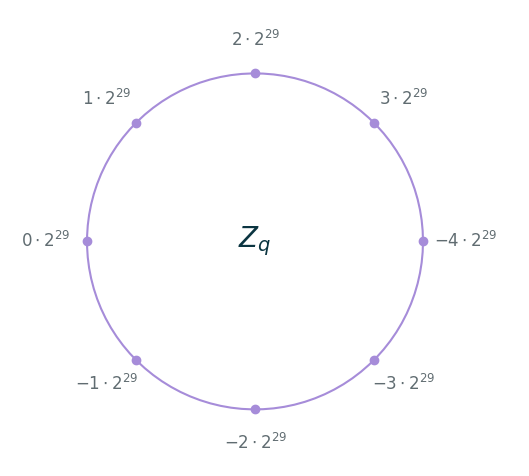
\includegraphics[width=0.35\linewidth]{figures/bootstrap-ring}
	\caption{Ring for the above mentioned parameters, image taken from the blog.}
	\label{fig:bootstrap-ring}
\end{figure}

Consider the function $F(b_0, b_1)$, where both inputs are LWE ciphertexts:
\begin{center}
	$F(b_0, b_1) = \text{Encode}(-3) - b_0 - b_1$. 
\end{center}
Looking at the function and the ring above, the function starts at Encode(3) = $-3 \cdot 2^{29}$ and essentially just moves two dots anti-clockwise for each $b_i = Encrypt(2)$ (meaning, it is true).
\begin{displaymath}
	F(b_0, b_1) = 
	\begin{array}{|c|c|c|}
		\hline
		b_0 & b_1 & F(b_0, b_1) \\ \hline
		Encode(2) & Encode(2) &  Encode(1) \\ \hline
		Encode(2) & Encode(0) & Encode(3) \\ \hline
		Encode(0) & Encode(2) & Encode(3) \\ \hline
		Encode(0) & Encode(0) & Encode(-3)  \\ \hline
	\end{array}
\end{displaymath}

Note that when when both $b_0$ and $b_1$ are Encode(2), $-2 \cdot 2^{29} < F(b_0, b_1) < 2 \cdot 2^{29}$. We can define a step function such that:
\begin{center}
	\begin{equation}
		Step(x) = 
		\begin{cases}
			0 \quad \text{if } -q/4 < x \leq q/4  = -2 \cdot 2^{29} < x \leq 2 \cdot 2^{29}\\
			Encode(2) \quad otherwise
		\end{cases}
	\end{equation}
\end{center}
Then, Step(F($b_0, b_1$)) is basically the NAND operation.

\begin{displaymath}
	Step(F(b_0, b_1)) = 
	\begin{array}{|c|c|c|c|}
		\hline
		b_0 & b_1 & F(b_0, b_1) & Step(F(b_0, b_1)) \\ \hline
		Encode(2) & Encode(2) &  Encode(1) & Encode(0) \\ \hline
		Encode(2) & Encode(0) & Encode(3) & Encode(2) \\ \hline
		Encode(0) & Encode(2) & Encode(3) & Encode(2) \\ \hline
		Encode(0) & Encode(0) & Encode(-3)  & Encode(2) \\ \hline
	\end{array}
\end{displaymath}

Therefore, we can say that NAND($l_0, l_1$) = Step(F($b_0, b_1$)) = Step($\text{Encode}(-3) - b_0 - b_1$).\\
The subtraction methods defined above can be used to calculate the value of F, and bootstrap can be used to calculate the Step function. Thus, this operation becomes equivalent to Bootstrap(CSub(Encode(-3), CSub($b_0, b_1$))). Here, -3 becomes a trivial LWE ciphertext instead of plaintext.

\section{Bootstrap: Building the Step Function}
Consider a polynomial $t(x) = -1 - x - x^2 - ... - x^{N/2 - 1} + x^{N/2} + x^{N/2 + 1} + ... + x^{N-1}$, where N/2 coefficients are -1 and the other half are 1. We call this the test polynomial. Now, if this is rotated by 1:
\begin{center}
	$\text{IntRotate}(1, t(x)) = x \cdot t(x) = -1 -x -.....- x^{N/2} + x^{N/2 + 1} + ....+ x^{N/2}$
\end{center}

\begin{minted}[
	fontsize=\small,
	frame=single,
	framesep=3mm,
	bgcolor=bg
	]{python}
def generate_tx(N) -> Polynomial:
	'''
	This function generates the polynomial i(t).
	'''
	# building the polynomial
	tx_coeffs = np.ones(N, dtype=np.int32)
	# updating the first half to be -1
	tx_coeffs[:N//2] = -1
	tx_poly = Polynomial(N, tx_coeffs)
	return tx_poly
\end{minted}

This rotates the coefficients one place to the right. The coefficient of $x^{N-1}$ comes to the front with a - sign. Meaning, now, there are N/2 + 1 coefficients that are -1 and N/2 - 1 that are 1. Now, if we keep rotating it, such that we rotate it by N/2:
\begin{center}
	$\text{IntRotate}(N/2, t(x)) = -1 - x -....- x^{N-1}$
\end{center}
All the coefficients are -1. Rotating it one more time would result in a polynomial:
\begin{center}
	$\text{IntRotate}(N/2 + 1, t(x)) = 1 - x - x^2 - ...- x^{N-1}$
\end{center}
Rotating it N times results in all the coefficients becoming positive. So, if we were to try and just look at the coefficient of the constant term ($x^0$), we can generalize it as follows:
\begin{equation}
	\text{Coeff}(0, \text{IntRotate}(i, t(x))) = 
	\begin{cases}
		-1 \qquad \text{if } 0 \leq i \leq N/2 \\
		 1 \qquad \quad \text{if } N/2 < i \leq N
	\end{cases}
\end{equation}
This equation can be further generalized to include \text{cases} when i is negative, which is also possible
\begin{equation}
	\text{Coeff}(0, \text{IntRotate}(i, t(x))) = 
	\begin{cases}
		-1 \qquad \text{if } -N/2 \leq i \leq N/2 \\
		1 \qquad \quad \text{otherwise}
	\end{cases}
\end{equation}

Also, from the blind rotate section, we know:
\begin{center}
	$\text{Rotate}(i, f(x)) = \text{IntRotate}(\lfloor \frac{2N}{q} \cdot i \rceil, f(x))$
\end{center}

So we can replace the IntRotate function with the Rotate function (because a. its defined for ciphertexts, and b. it will the change the limits from N to q, which is what we have when working with ciphertexts):
\begin{equation}
	\text{Coeff}(0, \text{Rotate}(i, t(x))) = 
	\begin{cases}
		-1 \qquad \text{if } -q/4 \leq i \leq q/4 \\
		1 \qquad \quad \text{otherwise}
	\end{cases}
\end{equation}

The above equation looks very similar to the step function, it has the same conditions for the input, but the output differs as this outputs -1 or 1 and step function outputs Encode(2) or 0. We can modify the above function to get the output of Step like this:
\begin{center}
	$\text{Step}(i) = \frac{\text{Encode(2)}}{2} + \text{Coeff}(0, \text{Rotate}(i, \frac{\text{Encode(2)}}{2} \cdot t(x)))$
\end{center}
Remember that Encode(2) is not a plaintext but a trivial LWE encryption of 2. This way, we have the step function implemented as bootstrap, and it utilizes BlindRotate and Coeff (ExtractSample) functions to implement it homomorphically.

\begin{minted}[
	fontsize=\small,
	frame=single,
	framesep=3mm,
	bgcolor=bg
	]{python}
def create_trivial_rlwe_ciphertext(mx: Polynomial, config: RLWEConfig):
	'''
	This function creates a trivial RLWE ciphertext. A trivial RLWE ciphertext is one where the polynomial is one where b is the polynomial itself while a is a zero polynomial.
	'''
	a = make_zero_polynomial(config.N)
	return RLWECiphertext(a, mx, config)
	
def create_trivial_lwe_ciphertext(m: LWEPlaintext, config: LWEConfig):
	'''
	This function creates a trivial LWE ciphertext, which is an LWECiphertext with a being a vector of zeros and b being the plaintext itself.
	'''
	a = np.zeros(config.n, dtype=np.int32)
	return LWECiphertext(a, m.m)
\end{minted}

\begin{minted}[
	fontsize=\small,
	frame=single,
	framesep=3mm,
	bgcolor=bg
	]{python}
def bootstrap(i: LWECiphertext, bsk: BootstrapKey, R:RLWECiphertext, scale_lwe: LWECiphertext):
	'''
	This function implements the bootstrap function to calculate the step operation defined above for the input i. The bsk is the bootstrapping key.
	This function returns 0 if i is in (-q/4, q/4], else, it returns an lwe encryption of scale.
	NOTE [IMPORTANT]: Note that if scale is the cleartext np.int32 value, scale_lwe encrypts Encode(scale)/scale.
	'''
	# blind rotate R
	rotated_rlwe = bsk.blindrotate(R, i)
	# extract sample to get the coefficient of constant
	coeff_lwe = extract_sample(0, rotated_rlwe)
	# adding scale_lwe to the output to get the offset-ed result of bootstrapping
	result_lwe = scale_lwe.add_ciphertext(coeff_lwe)
	
	return result_lwe
\end{minted}

\subsection{Details for FHE Implementation of Step using Boostrapping}
This section will describe the implementation details for the above defined operation. We want to implement bootstrap that evaluates the step function. Given an LWE ciphertext L (which will be the output of F described in the previous sections). The following things are needed:
\begin{itemize}
	\item $L \in \text{LWE}_s(i)$, an LWE encryption of i.
	\item $R \in \text{RLWE}_{s(x)}(\frac{\text{Encode}(2)}{2} \cdot t(x))$, a trivial RLWE encryption of the scaled test polynomial.
	\item $B \ in \text{LWE}_s(\frac{\text{Encode}(2)}{2}))$, a trivial LWE encryption.
\end{itemize}

Then, the bootstrap operation can be defined as: CAdd(B, ExtractSample(0, BlindRotate(L, R))).

\begin{minted}[
	fontsize=\small,
	frame=single,
	framesep=3mm,
	bgcolor=bg
	]{python}
def homomorphic_nand(b0: LWECiphertext, b1: LWECiphertext, constCipher: LWECiphertext, scale_lwe: LWECiphertext, txR:RLWECiphertext, bsk:BootstrapKey) -> LWECiphertext:
	'''
	This function implements the nand operation between two inputs b0 and b1 homomorphically.
	The way it does it is by first evaluating the value of F(b0, b1) = LWE(-3) - b0 - b1 and then running the bootstrap that implements the step function which evaluates the final nand function.
	Remember that 0 is equivalent to F while 2 is equivalent to T here. The output will be an LWE ciphertext encrypting 0 or 2 as well.
	constCipher is just the LWE Encryption of -3.
	'''
	# calculating constCipher - b0 - b1
	cc_minus_b0 = constCipher.sub_ciphertext(b0)
	F_lwe = cc_minus_b0.sub_ciphertext(b1)
	# call bootstrapping on this
	nand_lwe = bootstrap(F_lwe, bsk, txR, scale_lwe)
	
	return nand_lwe
\end{minted}

\chapter{TFHE and TFHE-rs: Introduction}
TFHE is a homomorphic encryption scheme. TFHE-rs is a rust library implemented by ZAMA that implements a variant of TFHE. TFHE follows the same methods and the ciphertexts mentioned in previous chapters. A few of its notable benefits are that it supports evaluation of small lookup tables using programmable bootstrapping, which it implements very efficiently and its runtime is fairly quick compared to other schemes. However. it has a few disadvantages. First, it can only work with small message sizes, meaning, the plaintext modulus (p) is fairly small). Second, the scale difference between p and q is huge (q is much larger), because of which, in vanilla TFHE, you have limited bit-widts to work with (usually 1 - 8 bits). \\
The TFHE-rs library attemps to and successfully solves this scale issue. On a higher level, does so by using multiple LWE ciphertexts to encrypt a single integer. It splits large integers (say a u64) into smaller blocks (say u8),  and each LWE ciphertext encrypts one block. The sequence of these blocks is important to extract the final integer out, and to ensure that, an encoding is used to preserver that sequence. The library abstracts all the internal math of this sequence of LWE ciphertexts so that the user can focus directly on arithmetic.
\begin{figure}[H]
	\centering
	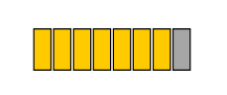
\includegraphics[width=0.3\linewidth]{figures/single_lwe}
	\captionsetup{justification=centering}
	\caption{LWE encryption of one block (image taken from the \href{https://github.com/zama-ai/tfhe-rs-handbook}{TFHE-rs Handbook}).\\
	The yellow blocks represent the a component (array of size n), and the grey block is the b component for LWE encryption}
	\label{fig:singlelwe}
\end{figure}

\begin{figure}[H]
	\centering
	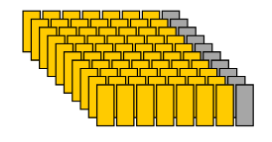
\includegraphics[width=0.3\linewidth]{figures/overall_lwe}
	\captionsetup{justification=centering}
	\caption{Encryption of larger scale integer using LWE blocks (each 'row' is an LWE block; image taken from the \href{https://github.com/zama-ai/tfhe-rs-handbook}{TFHE-rs Handbook})}
	\label{fig:overalllwe}
\end{figure}

\section{TFHE: Setup and Introduction}
TFHE, as stated above, is an encryption scheme which is also based on (G)LWE ciphertexts. Where it is different from other schemes is that TFHE implements a very efficient bootstrapping operation (orders of magnitude faster than other schemes afaik), and this bootstrapping is also programmable, meaning, in addition to resetting the noise in the ciphertext, it can also evaluate a function on it and return the encrypted output of the function, which is why it is often referred to as \textit{programmable bootstrapping (PBS)} or \textit{functional bootstrapping}.\\
One thing to note is that multiplication is not natively available in TFHE (compared to something like CKKS, which allows multiplication by design). However, PBS can be used to perform multiplication, whcih converts it from an additive scheme to a fully homomorphic encryption scheme.\\

\textbf{NOTE ABOUT NOTATION:} In this and the coming chapters, a polynomial will be denoted by an uppercase letter, while a constant will be denoted by a lowercase letter. Vectors of elements will be denoted by bold letters based on their corresponding types (I will try my best to follow this bold thing, but I might forget, that will not be a problem because I will most definitely mention that that particular letter references a vector of a specific element).

\subsection{Hard Lattice Problems: LWE and GLWE Assumptions}
TFHE and most other homomorphic encryption schemes are based on a family of hard problems, the \textbf{LWE (Learning With Error)} problem. This is what ensures its security. Basically, it can be thought of as something similar to solving a system of noisy linear equations. This problem is of two types: a search problem and a decision problem.

\subsubsection{LWE: Learning With Errors}
\textbf{Let:}\\
\begin{itemize}
	\item $n \in N$, a positive integer called the LWE dimension,
	\item $q \in N$, a positive intger, called the ciphertext modulus,
	\item $\textbf{s} = (s_0, s_1, ..., s_{n-1}) \in R_q^n$ be a vector that is obtained from a distribution $\mathcal{D}$ known as the secret distribution. Conversely, \textbf{s} is called the secret, \footnotemark{}
	\item a distribution $\chi$ called the noise distribution.
\end{itemize}
Then, a sample from this LWE distribution that is defined using all these parameters is denoted by $\text{\textit{LWE}}_{n, q, \chi, \mathcal{D}}$. Additionally, a point sampled from this distribution looks like:
\begin{center}
	$(a, b = \sum\limits_{i=0}^{n-1}a_i \cdot s_i + e_i) \in \mathbb{Z}_q^{n+1}$
\end{center}
where, $\textbf{a} = (a_0, a_1, ..., a_{n-1}) \in \mathbb{Z}_q^n$ is a vector sampled from a uniform distribution $\mathcal{U}(\mathbb{Z}_q)$\footnotemark[\value{footnote}].\\
This is the LWE distribution, and as mentioned above, there can be two different problems made out of this:
\begin{itemize}
	\item \textbf{Search Problem:} This problem is about trying to find out the secret vector \textit{s} from a number of samples generated from $\text{\textit{LWE}}_{n, q, \chi, \mathbb{D}}$.
	\item \textbf{Decision Problem:} In this problem, we try to distinguish between samples from the $\text{\textit{LWE}}_{n, q, \chi, \mathbb{D}}$ and a uniform distribution $\mathcal{U}(\mathbb{Z}_q)$.
\end{itemize}

The security of encryption schemes that use either of these LWE problems as their basis depend of the values of q, n, distributions $\chi$ and $\mathcal{D}$. Additionally, the security of an LWE based ciphertext is denoted by something called as the \textit{security factor} which is denoted by $\lambda$. For a scheme with a specific configuration to have a security level $\lambda$, breaking it should require atleast $2^\lambda$ operations. $\lambda = 128$ is considered to be a good value to ensure secruity of such systems. \vspace{5em}

\footnotetext{Every element of the array is independently sampled from its distribution.}
\subsubsection{GLWE: General Learning With Errors}
The problem with LWE is that is works with integers, and LWE ciphertexts also have a high expansion factor between plaintext and ciphertext (there is a large difference between magnitudes of p and q). There can be instances where one needs to work with more complex structures such as polynomials, and for that, the General Learning With Errors problem is more suitable,  as instead of encrypting and working with integers, it works with polynomials in a ring $R_q[X] / (X^N + 1)$. Since it works with a polynomial, it uses more complex mathematical operations than integers. It is important to remember that in GLWE, the coefficients of polynomials are modulus q, and the polynomials themselves are modulus $(X^N + 1)$, meaning, their maximum degree is N-1. This means that after any arithmetic operation, specifically multiplication, the resulting polynomial is reduced to a polynomial of degree N - 1 by taking mod wrt $(X^N  + 1)$, and the same goes for the coefficients where a modulus q operation is also applied on them (this is also done with LWE ciphertexts). \\
\textbf{Let:}
\begin{itemize}
	\item $k \in Z_+$, a positive integer, called the GLWE Dimension,
	\item $N \in Z_+$, a positive integer, called the polynomial size,
	\item $\chi$, the noise distribution,
	\item $\mathbb{D}$, the secret key distribution.
	\item $q \in Z_+$, a positive integer, the ciphertext modulus
\end{itemize}
Let $\textbf{S} = (S_0, S_1, ..., S_{k-1})$ be the vector of polynomials called the secret, where the coefficient for each polynomial $S_i$ is sampled from the secret distribution $\mathbb{D}$. Then, a sample from the GLWE distribution $\text{GLWE}_{q, k, N, \chi, \mathbb{D}}$ is defined as:
\begin{center}
	$\text{GLWE}_{q, n, N, \chi, \mathbb{D}} = (\textbf{A}, B = \sum\limits_{i=0}^{k-1} A_i \cdot S_i + E) \in \mathcal{R}_{q, N}^{k+1}$ \footnote{Remember that bold uppercase letters represent an array of polynomials, while lowercase bold letters represent an array of scalars.}
\end{center}
where, $\textbf{A} = (A_0, A_1, ..., A_{k-1})$ is an array of k polynomials, where each polynomial's coefficient is sampled from a uniform distribution $\mathcal{U}(\mathbb{Z}_q)$ independently, and the noise polynomial E has its coefficients sampled independently from the noise distribution $\chi$.\\
Like the LWE system, this also has two problem, which are same as the LWE ones but it works on polynomials:
\begin{itemize}
	\item \textbf{Search Problem:} Trying to find out the secret polynomial S from an arbitrary number of GLWE samples.
	\item \textbf{Decision Problem:} Trying to differentiate between samples from the RLWE distribution and points/polynomials sampled from the uniform $\mathcal{U}(\mathbb{R}_{q, N}^{k+1})$
\end{itemize}

Two important points:
\begin{itemize}
	\item For GLWE, if N = 1, k=n, then it becomes equivalent to the LWE system.
	\item If k = 1, then the resulting GLWE system is called the RLWE system (it works with 1 polynomial instead of an array of polynomials).
\end{itemize}


\section{FHE Ciphertext Types}
\subsection{LWE, RLWE \& GLWE Ciphertexts}
The LWE \& RLWE ciphertexts are what we looked at the previous chapters. The GLWE ciphertext is sort of a generalization of GLWE. Think of GLWE (this isnt how it literally happens, but I think its a good intuitive explanation) as sort of an RLWE encryption set but instead of the secret key and A being a single polynomial, they're an array of polynomials.\\
Given an encoded message polynomial $\tilde{M} \in R_q^n$, and a secret $\textbf{S} = (S_0, S_1, ..., S_{k-1}) \in R_{q, N}^k$, the GLWE encryption of the message is:
\begin{center}
	$CT = ((A_0, A_1, ..., A_{k-1}), B = \sum\limits_{i=0}^{i=k-1} A_i \cdot S_i + \tilde{M} + E) = GLWE_{\textbf{S}}(\tilde{M}) \in \mathcal{R}_{q, N}^{k+1}$
\end{center}

The random elements are sampled the same way as mentioned above in the GLWE system.\\
Note that while ideally, the coefficients of the noise polynomial E should be sampled independently, it is not mandatory, but ideally, this property would be there. Additionally, the different coefficients can be sampled from different noise distributions $\mathcal{D}$.

\subsection{Lev, RLev \& GLev Ciphertexts:}
These are a family of more complex ciphertexts that can be used for some applications downstream. They are actually a collection of GLWE ciphertexts, but they have two additional parameters, \textit{a decomposition base} and \textit{a decomposition level}. These ciphertexts do not encode a plaintext (encoded message), but rather, the cleartext raw message itself, and thus, assumes that the raw message is much smaller compared to the ciphertext modulus.\\
Given the GLWE secret key \textbf{S}, the ciphertext modulus \textit{q}, a decomposition level $l \in \mathbb{N}$ and a decomposition base $\mathcal{B} \in N$, the GLev ciphertext encrypting a cleartext message M (not encoded) is a collection of GLWE ciphertexts under the same configurations:
\begin{center}
	$CT_{Glev} = \text{GLev}_\textbf{S}^{\mathcal{B}, l} (M) = (CT_0, CT_1, ..., CT_{l-1}) \in \mathcal{R}_{q, N}^{l \cdot (k+1)}$
\end{center}
where each ciphertext $CT_i$ is an GLWE CIphertext such that:
\begin{center}
	$CT_i = GLWE_\textbf{S} (\frac{q}{\mathcal{B}^{(i+1)}} \cdot M) \in \mathcal{R}_{q, N}^{k+1} \qquad \forall \quad 0 \leq i < l$ 
\end{center}

When N = 1 and k = n, the resulting ciphertext is called Lev (think of its a LWE equivalent for GLev), and when N>1 and k=1, then its called an RLev (think of it as RLWE  equivalent of GLev).

\subsection{GSW, RGSW \& GGSW Ciphertexts}
On a high level, GGSW ciphertexts are a collection of GLev ciphertexts that use elements of secret key to define the GLev plaintexts. This sounds very vague but the mathematical definition itself does a good job of explaining what they are in my opinion. 
Given the decomposition base $\mathcal{B}$, the decomposition level \textit{l}, and the GLWE secret key $\textbf{S} = (S_0, S_1, ..., S_{k-1})$, the GGSW ciphertext is defined as:
\begin{center}
	$GGSW_\textbf{S}^{\mathcal{B}, \textit{l}}(M) = (CT_0, CT_1, .., CT_k) \in \mathcal{R}_{q, N}^{(k+1)^2 \cdot l}$
\end{center}
such that:
\begin{center}
	$CT_i = GLev_\textbf{S}^{\mathcal{B}, \textit{l}} (-S_i \cdot M) \in R_{q, N}^{(k+1) \cdot l} \qquad \forall \quad 0 \leq i \leq k$
\end{center}

\section{Encoding and Decoding}
The encoding and decoding methods for TFHE are almost the same as that discussed above. However, there is a very small difference, that is, you can have padding bits in TFHE.
\subsection{What does padding mean?}
Generally, there are two things defined, p: plaintext modulus and q; ciphertext modulus, and to encode a message, you multiply it with $\Delta = \frac{q}{p}$. What happens in padding is that in addition to p and q, a value $\pi > 0$ called the padding size is defined. The value of $\Delta$ now changes to $\Delta = \frac{q}{p \cdot 2^\pi}$. 

\begin{figure}[H]
	\centering
	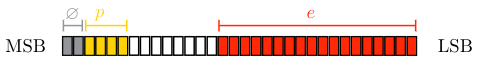
\includegraphics[width=0.3\linewidth]{figures/padding-encoding}
	\captionsetup{justification=centering}
	\caption{Representation of plaintext when padding is used. Here, padding is set to be 2 bits ($\pi = 1$). \\
		Image taken from the TFHE-rs Handbook}
	\label{fig:padding-encoding}
\end{figure}

\subsection{Why is padding used?}
While it might look like padding wastes valuable space, it is important for applications such as PBS. This is because padding allows us to implement PBS based table lookups for non-negacyclic functions. Without it, youd be stuck to working only with negacyclic functions, while in reality, many functions are not negacyclic. Having a padding bit, and most importantly, having the padding bit known (as in what value it holds) allows one to go for non-negacyclic functions. Typically, the value in the padding bit is kept to zero.

\subsection{Carry Bits}
We want the value in the padding bit(s) to be known (generally 0). But during some arithmetic operations, it is possible that the resulting message has a higher bit width and it goes beyond the plaintext modulus p and modifies the value of the padding bit. For example, assume that $p = 2^2$, and you have two messages, $m_1 = 2 = 01_2$, and $m_2 = 3 = 11_2$. Adding them both gives $5 = 101_2$, which would definitely change the value of the padding bit from 0 to 1, and that would result in an inaccurate PBS operation. To prevent this unwanted (unless its explicitly done) updating, carry bits are used. Two things are defined:
\begin{itemize}
	\item Message Modulus, \textbf{msg}
	\item Carry Modulus, \textbf{carry}
\end{itemize}
such that $\text{\textbf{carry}} \cdot \text{\textbf{msg}} = p$. The message modulus sets the range for the actual cleartext message. \\
This ensures that even if the result of the output goes beyond the message modulus, it can never edit the padding bit, ensuring accurate bootstrapping. Once the carry space becomes full, a PBS operation be done, to reduce the message modulus wrt \textbf{msg}, which resets the carry bits. \newline

(Thoughts to myself: Okay if you eventually have to take modulus once the carry bit is full, can you not also do the same for when the padding space gets edited? That removes the need for shrinking the actual message space. I can think of the following reasons:)
\begin{itemize}
	\item If the parameters are set correctly, then this situation never arises, unless something crazy happens. This is more of a foolproof safety check.
	\item This PBS operation is hard and you want to delay it as long as possible.
\end{itemize}

\section{Encoding Booleans}
Booleans (1/0; T/F) can be represented using integers, 0 for False/0, 2 for True/1 for example, and then they can be encoded the same way as ints.

\section{Simple Operations on TFHE Ciphertexts}
Simple arithmetic operations such as addition and multiplication with a scalar and addition with another ciphertext is done the same way as stated in the previous chapters for GLWE ciphertexts. For GGWE \& GLev ciphertexts, since theyre essentially sequences of GLWE ciphertexts, these operations from GLWE can be trivially done by performing those operations on the corresponding GLWE building blocks.

\section{Key Switching}
For any operation that needs to be done between two ciphertexts, it is important that theyre encrypted using the same secret key. Ciphertexts encrypted under different secret keys can not be correctly added, multiplied etc even if their shapes are the same. To be able to do things like these, the key switching operation is done. If you have a ciphertext $CT_{in} = \text{GLWE}_{\mathbf{S_{in}}}(M)$, using key switching, you can get another ciphertext $CT_{out} = \text{GLWE}_\mathbf{S_{out}}(M)$, that is encrypted under a different key compared to the input ciphertext. Note that this 'switched' key can have different parameters such as N, q etc than the input secret key. There any many different ways/algorithms for key switching, and all of them requires something called as the keyswitching keys. However, intuitively, keyswtiching keys are encryptions of the input ciphertext's key $\mathbf{S_{in}}$ using the output secret key $\mathbf{S_{out}}$.\\
Note that the previous chapters talk about switching keys between different ciphertexts. This section will take about other algorithms, specific to TFHE.

\subsection{Radix Decomposition}
Radix Decomposition is a part of most key switching operations. Radix decomposition is defined for an integer $x \in Z_q$. For a given decomposition base $\mathcal{B}$ and decomposition level \textit{l}, such that $\mathcal{B}^\mathit{l}$ divides q. The idea is to decompose x into a vector $(x_1, x_2, ..., x_l)$, such that:
\begin{center}
	$\langle (x_1, x_2, ..., x_l), (\frac{q}{\mathcal{B}}, \frac{q}{\mathcal{B}^2}, ..., \frac{q}{\mathcal{B}^\mathit{l}}) \rangle = \sum\limits_{i=1}^{\mathit{l}} x_i \cdot \frac{q}{\mathcal{B}^i} = \lfloor x \cdot \frac{q}{\mathcal{B}^\mathit{l}} \rceil \cdot \frac{q}{\mathcal{B}^\mathit{l}} \in \mathbb{Z}_q$
\end{center}
Note that $\langle ., . \rangle$ represents the dot product between the two. (Also, while the above equality might look daunting, the right hand side of the equality should equate to x or something extremely close to x if everything is correct and the parameters are right.)

It is implemented in TFHE-rs using an algorithm called BalDecomp$^{\mathcal{B}, l}$(x)

\subsection{LWE and GLWE Key Switch}
\subsubsection{LWE Key Switch}
The LWE Key Switch operation takes as input an LWE ciphertext encrypting a plaintext under the a secret key $\mathbf{s} = (s_0, s_1, ..., s_{n-1})$, and outputs a GLWE ciphertext encrypting the same plaintext under a secret key $\mathbf{S} = (S_0, S_1, ..., S_{k-1})$. In the case when N = 1, then the output of this key switch operation becomes an LWE ciphertext. Additionally, this function also requires a keyswitch key, which is an array of GLev ciphertexts where each element encrypts a single element of \textbf{s}:
\begin{center}
	$\text{KSK} = \{CT_i: GLev_\mathbf{S}^{\mathbb{B}, \mathit{l}}(s_i)\}_{0 \leq i \leq n-1} $
\end{center}
Algorithm to perform this keyswitch is as follows:
\begin{figure}[H]
	\centering
	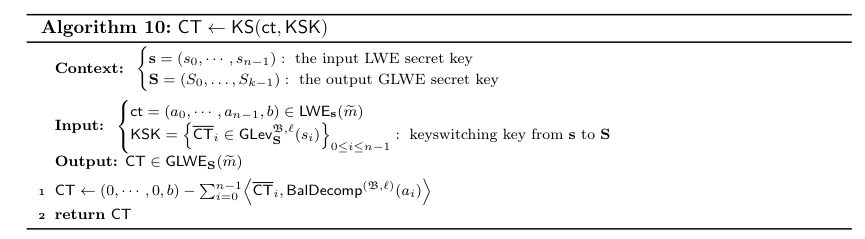
\includegraphics[width=1.0\linewidth]{figures/LWE-KS}
	\caption{LWE Keyswitching algorithm, image taken from the TFHE-rs handbook.}
	\label{fig:lwe-ks}
\end{figure}

\subsubsection{GLWE Key Switch}
The GLWE keyswitch takes as input a GLWE ciphertext encrypted under a GLWE key $\mathbf{S_{in}}$ and outputs another GLWE ciphertext encrypting the same message under a different GLWE key $\mathbf{S_{out}}$. The keyswitch key here is a sequence of GLev ciphertextws encrypting individual polynomials of $\mathbf{S_{out}}$ using the $\mathbf{S_{in}}$.
\begin{center}
	$\text{KSK} = \{\text{CT}_i: GLev_{\mathbf{S_{in}}}^{\mathcal{B}, \mathit{l}} (S_{in, i})\}_ {0 \leq i \leq k_{in}-1}$
\end{center}

The algorithm for this keyswitch operation is as follows:
\begin{figure}[H]
	\centering
	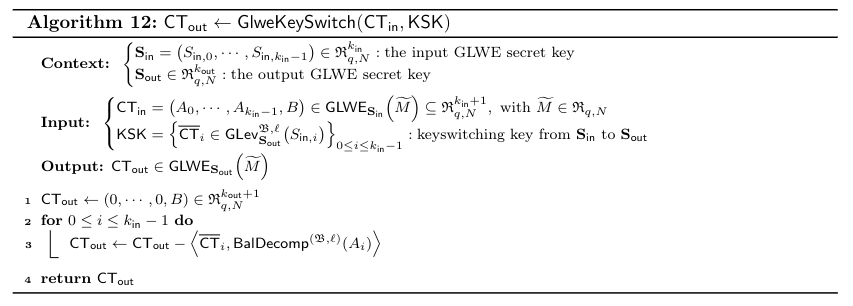
\includegraphics[width=1.0\linewidth]{figures/GLWE-KS}
	\caption{GLWE keyswitching algorithm, taken from the TFHE-rs handbook.}
	\label{fig:glwe-ks}
\end{figure}

\subsection{Packing Key Switch}
Packing is the process of taking many LWE ciphertexts and 'packing' them into one GLWE ciphertext, this works because a GLWE ciphertext encrypts a polynomial. Basically, if you have LWE ciphertexts that encrypt a collection of numbers, say $(l_0, l_1, ..., l_{N-1})$, then the packing will result in a GLWE ciphertext that encrypts a polynomial $l_0 + l_1x + ... + l_{N-1}x^{N-1}$.\\
The packing key switch operation takes a collection of $\alpha < N$ LWE ciphertexts $\{ ct_0, ct_1, ..., ct_\alpha-1 \}$, encrypted under an LWE key \textbf{s} and a set of $\alpha$ indices for these ciphertexts, $\alpha = \{i_j\}_{j=0}^{j=\alpha - 1}$ and returns a GLWE ciphertext that encrypts a polynomial where the coefficients are the messages encrypted in the input LWE ciphertexts. \\
Here, the keyswitch key again is the GLev encryption of the LWE key \textbf{s} using the GLWE key \textbf{S}. The algorithm to perform this operation is given below:
\begin{figure}[H]
	\centering
	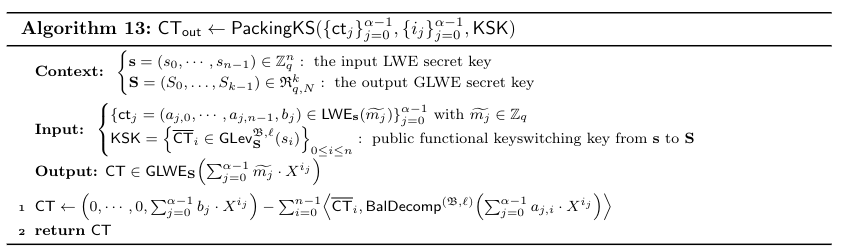
\includegraphics[width=1.0\linewidth]{figures/Packing-KS}
	\caption{Algorithm to perform packing key switching. Image taken from the TFHE-rs handbook.}
	\label{fig:packing-ks}
\end{figure}

\section{Programmable Bootstrapping (PBS): Building Blocks}

\subsection{Modulus Switching}
The modulus switch operation switches the ciphertext modulus of an encrypted ciphertext from existing q to a new modulus w. If you have a ciphertext that encrypts an encoded message $\tilde{m}$ (encoded using q), the output of this operation returns a ciphertext that is encoded in w: $\lfloor \tilde{m} \cdot \frac{w}{q} \rceil$. For TFHE's PBS, w is set to be 2N. There are 3 types of modulus switching operations, which are controlled by the parameter $\text{pfailMitigationTechnique}$:
\begin{itemize}
	\item $\text{pfailMitigationTechnique}$ = 0: No mitigation technique used, no drift mitigation key needed, classical modulus switching is used.
	\item $\text{pfailMitigationTechnique}$ = 1: Mean compensation technique used for which no drift mitigation key is needed, after that, classical modulus switching is used.
	\item $\text{pfailMitigationTechnique}$ = DMK: Drift mitigation technique is used before performing modulus switching. Drift Mitigation Key (DMK) needed.
\end{itemize}

The modulus switching algorithm:
\begin{figure} [H]
	\centering
	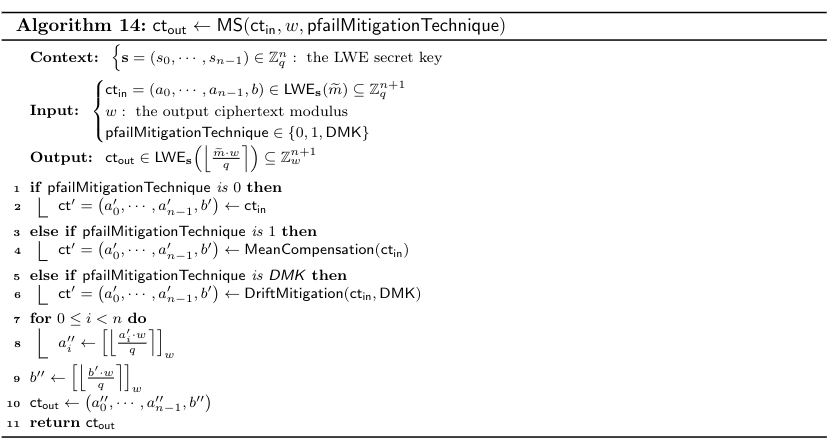
\includegraphics[width=1\linewidth]{figures/modulus-switching}
	\caption{Modulus Switching Algorithm, image taken from the TFHE-rs handbook.}
	\label{fig:modulus-switching}
\end{figure}

\subsubsection{Mean Compensation}
Decrypting a ciphertext produces a noisy version of the encoded ciphertext (because it returns m + e, and not just m). This is then decoded to get the original message. However, there is a chance that the decryption and decoding fail, which is called the failure probability. This probability is directly influenced by the magnitude of noise int he ciphertext (higher the noise, higher this probability). Also, during the process of modulus switching, the noise comes from rounding and the resulting rounding errors. The drift vector is just a vector of these rounding errors that happen during modulus switching.\\
The mean compensation technique aims at reducing this noise by 'adjusting' the mean of this drift vector to zero.
\begin{figure}[H]
	\centering
	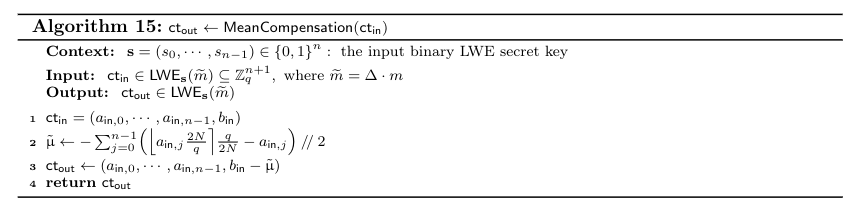
\includegraphics[width=1.0\linewidth]{figures/mean-compensation}
	\caption{Mean Compensation Algorithm, image taken from the TFHE-rs handbook.}
	\label{fig:mean-compensation}
\end{figure}

\subsubsection{Drift Mitigation}
Drift Mitigation is an alternative to Mean Compensation for reducing noise during the modulus switching operation. The idea here is that, the rounding error is dependent on the input mask (\textbf{a}). Adding a 0 LWE ciphertext to the input randomizes this mask and thus the rounding error. While this also adds a little extra noise (as youre adding two LWE ciphertexts), this is okay as the rounding noise reduction is much higher than the added noise. To perform this operation, an extra key, called the Drift Mitigation Key (DMK) is required, which are essentially fresh LWE encryptions of 0. $\text{DMK} = \{ ct_z = \text{LWE}(0) \}_{z \in [1, Z]}$.\\
Drift Mitigation Algorithm:
\begin{figure}[H]
	\centering
	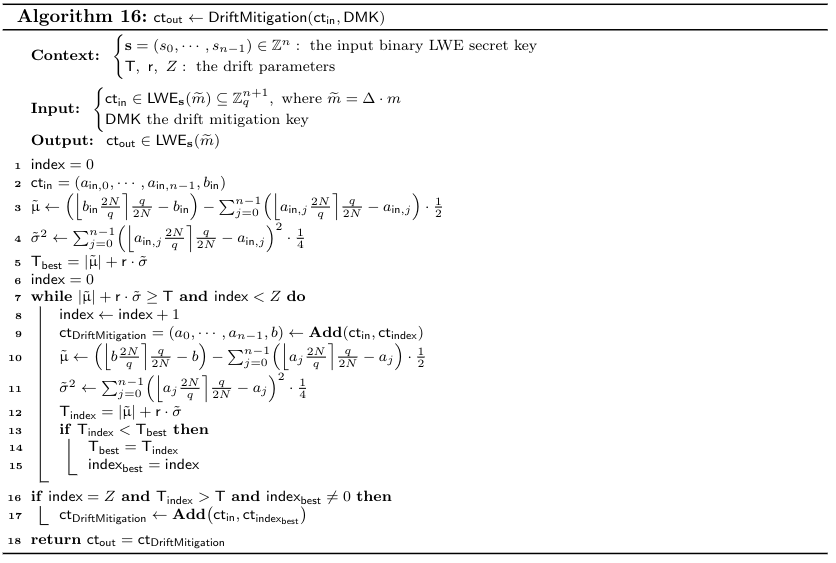
\includegraphics[width=1.0\linewidth]{figures/drift-mitigation}
	\caption{Drift Mitigation Algorithm, image taken from the TFHE-rs handbook.}
	\label{fig:drift-mitigation}
\end{figure}

\subsection{External Product}
External product essentially is the ciphertext-ciphertext mulitplication. Like shown in the previous chapters, where we performed multiplication between a GSW and an RLWE ciphertexts, here, we generalize it to GGSW and GLWE ciphertexts. Instead of using the base-p representation for RLWE ciphertext, we use the BalDecomp (Balanced Radix decomposition).
\begin{figure}[H]
	\centering
	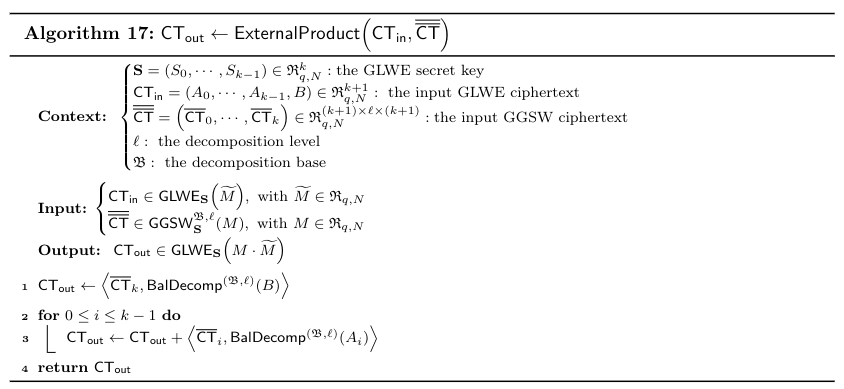
\includegraphics[width=1.0\linewidth]{figures/CMul}
	\caption{External Multiplication Algorithm, image taken from the TFHE-rs handbook.}
	\label{fig:cmul}
\end{figure}

\subsection{CMux}
The CMux operation is also extremely similar to what we saw previously, except that now, it works with more general GLWE and GGSW ciphertexts.
\begin{figure}[H]
	\centering
	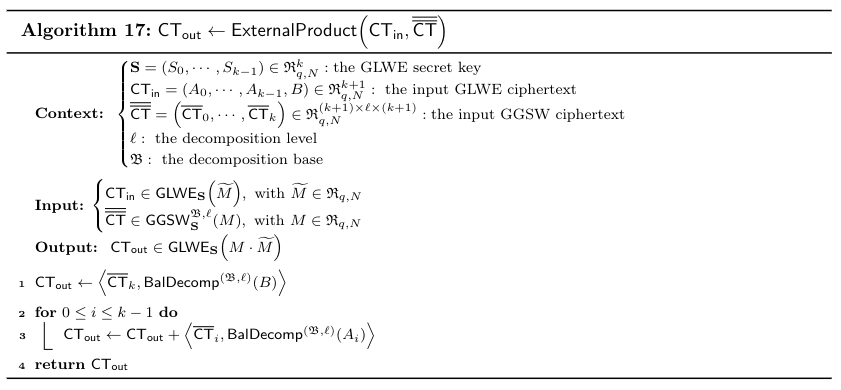
\includegraphics[width=0.9\linewidth]{figures/Cmux}
	\caption{CMux Algorithm for TFHE, image taken from the TFHE-rs handbook.}
	\label{fig:cmux}
\end{figure}

\subsection{Blind Rotate}
The blind rotate operation, just like the other operations, is similar in how its done in the previous chapters, except that the ciphertexts are the general versions. The bootstrapping key is a sequence of GGSW ciphertexts that encrypts each component of the LWE encryption key.
\begin{figure}[H]
	\centering
	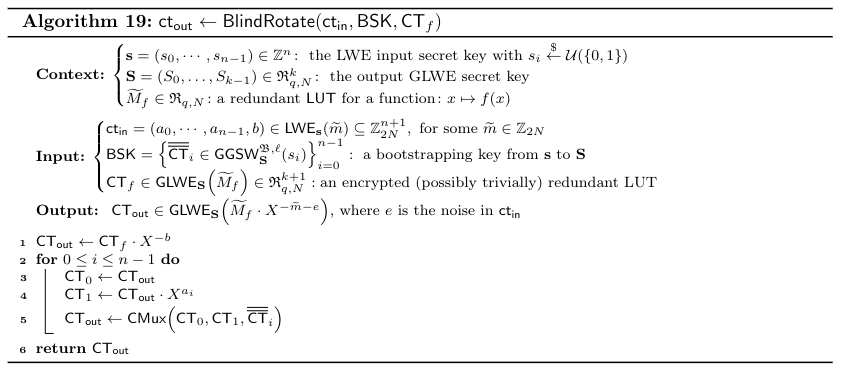
\includegraphics[width=1.0\linewidth]{figures/BlindRotate}
	\caption{BlindRotate Algorithm, image taken from the TFHE-rs handbook.}
	\label{fig:blindrotate}
\end{figure}

\section{Programmable Bootstrapping}
The programmable bootstrapping in TFHE achieves two things:
\begin{itemize}
	\item It refreshes noise of the output ciphertext (noise of the output is independent of the input ciphertext).
	\item It allows one to evaluate a function on the input ciphertext and return the output of that function encrypted as an LWE ciphertext.
\end{itemize}
While the PBS implementation is similar to the ones in the previous chapters, one big difference is its ability to evaluate a function, for which, it takes as input, something known as a redundant LUT. 
\begin{figure}[H]
	\centering
	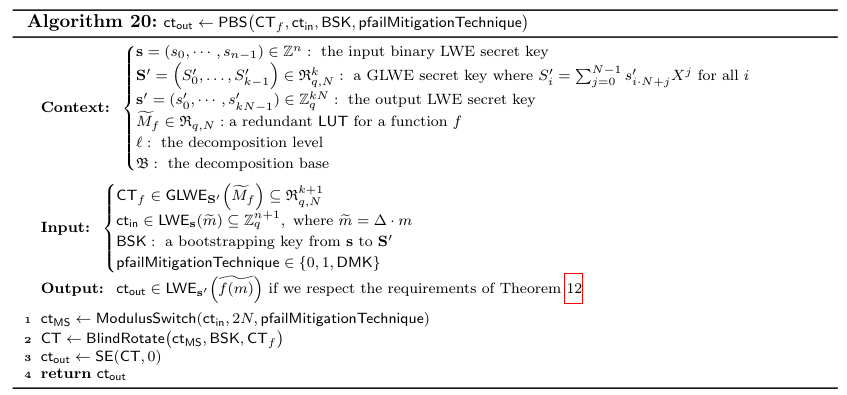
\includegraphics[width=1.0\linewidth]{figures/PBS}
	\caption{PBS Algorithm, image taken from the TFHE-rs handbook.}
	\label{fig:pbs}
\end{figure}

Let $\textbf{s} = (s_0, s_1, ..., s_{n-1})$ be the LWE encryption key for the input, and $\textbf{S}' = (S'_0, S'_1, ..., S'_{k-1})$ be the GLWE encryption key, and the corresponding flattened LWE secret key $\textbf{s}' = (s'_0, s'_1, ..., s'_{kN - 1})$ s.t  $S'_i = \sum\limits_{j=0}^{N-1} s'_{i \cdot N + j} \cdot X^j$. The BSK is the associated bootstrapping key from \textbf{s} to \textbf{S}`. For an LWE ciphertext encrypting an encoded message $\tilde{m} = m \cdot \Delta$ for some $m \in Z_{2p}$ for some p dividing N and $\Delta = \frac{q}{2p}$. $\widetilde{M_f}$ is the $\frac{N}{p}$-redundant LUT for a function $f: Z_p \rightarrow Z_q$ and let $\text{CT}_f$ be a trivial RLWE encryption of $\widetilde{M_f}$. These are the inputs to the bootstrap operation alongisde the LWE ciphertext.

\subsubsection{Redundant Lookup Table (LUT)}
A redundant LUT is an LUT that encodes a function $f$ (encodes, not encrypts), and the entries (outputs I think) of this function are stored as coefficients of a polynomial in $\mathcal{R}_{q, N}$. The redundancy comes from storing entries $f(i)$ r times with a certain shift. The term mega-cell is used to denote each block of redundant values in an r-redundant lookup table.
\begin{center}
	$\widetilde{M_f} = X^{-r/2} \sum\limits_{i=0}^{N/r - 1}  X^{i \cdot r} \cdot \left (\sum\limits_{j=0}^{r-1} \widetilde{f(i)} \cdot X^j \right )$
\end{center}
$\widetilde{f(i)}$ is an encoding of the function output $f(i)$. Another way to write this LUT is just using the mega cell values:
\begin{center}
	$\left [ \widetilde{f(0)}, \widetilde{f(1)}, ..., \widetilde{f(\frac{N}{r} - 1)} \right ]$
\end{center}

Note that this is the basic PBS operation. There are other types of PBS operations that have their own characteristics.


\chapter{References}
\begin{itemize}
  \item \href{https://docs.zama.org/tfhe-rs/references/core-crypto-api/tutorial}{Core-crypto - TFHE-rs}
  \item \href{https://www.daniellowengrub.com/blog/2024/01/03/fully-homomorphic-encryption}{Daniel Lowengrub's Blog on TFHE implementation from scratch.} \label{ref:blog}
  \item \href{https://github.com/zama-ai/tfhe-rs-handbook}{The TFHE-rs Handbook.(Read until the PBS section, it describes a lot of other stuff too.)} \label{ref:handbook}
   \item \href{https://docs.zama.org/tfhe-rs/explanations/tfhe-deep-dive}{TFHE-rs's blog series: TFHE Deep Dive}
   \item \href{https://hal.science/hal-04121360/document}{Hitchhiker's Guide to the TFHE Scheme (havent gone through yet)}.
\end{itemize}

\end{document}
